\chapter{Grant-Free Access via Riemannian Blind Signal Recovery} \label{rocma:chap}

%connecting ideas
%1) why WF is not enough? point to missing convergence guarantees, or worst-case proof
%2) Can we do better? are there other geometrical perspectives that we can use to exploit /improve blind recovery?

In the previous chapter, we proposed a CMA-based source recovery method that uses regularization to recover multiple distinct source signals. 
Even when theoretical analysis and numerical simulations show satisfactory performance of WF-CMA, there are still aspects to be addressed.
First, there is still no theoretical guarantee that spectral initialization (or any other initialization method) would yield an initial iterate within the basin of attraction of the CMA cost function. In practical scenarios, the initialization could be inadequate in different channel conditions or settings. 
Second, we assumed that the number of active sources was known at the BS, which might not be true in practice and the BS would need to estimate the number of sources. 
Finally and more importantly, regularization usually requires parameter tuning for different realizations, and often increases computational complexity.  \crfootnote{Part of this chapter has been previously submitted to \textit{IEEE Transactions on Signal Processing} and is currently under review.}



%Unlike traditional stochastic gradient solutions that require large data samples, parameter tuning, and careful initialization, 

In this chapter, we explore a Riemannian optimization framework for blind multiple signal recovery. 
We leverage Riemannian geometry and encode the orthogonality requirement of recovered signals into a Riemannian manifold. This new search space transforms the original signal recovery problem into an unconstrained, regularization-free optimization problem over this Riemannian manifold. By exploiting efficient, low complexity solvers, this approach demonstrates full recovery of distinct source signals without special initialization or tuning, with high probability of success and modest sample complexity compared to traditional gradient descent approaches.


%First, the regularizing term typically requires to tune a scalar weight, e.g. $\gamma_0$ in Eq.(\ref{wfcma:eqn:cma_msr}), often by trial and error, with no performance guarantee under various possible scenarios.
%Second, different regularization approaches might lead to different solutions and performance, while no solution is consistently better than others. 
%Additionally, regularizing terms often increase the computation complexity as regularized cost functions would either require additional computations or delicate non-convex optimization steps. 
%Finally, regularizing terms proposed in the literature generally are limited to promote pairwise signal orthogonality instead of multi-lateral signal orthogonality, and also require more data samples to successfully suppress mutual interferences.


\section{Constrained Multiple Signal Recovery}
Figure~\ref{rocma:fig:system_model} depicts a blind signal recovery system, whose goal is to find multiple demixers that recover distinct source signals with minimal interference.
As stated in Section~\ref{system:ssec:blind_recovery}, CMA-based multiple source recovery requires additional constraints to ensure that the process actually accomplishes this task. Several works have proposed to add regularization term(s) to the cost function (\ref{system:eqn:cma_msr_orig}) to penalize against the recovery of identical signals by more than one solution vectors in $\widehat\W$.
For example, in \cite{Bessios1992mimocrimno,Li1998adaptivemimocma} the authors proposed adding a norm of joint cumulants for such source separation objective. 
Other proposals such as \cite{Nguyen1997} enforce orthogonality of the combiners at each gradient descent iteration, either via orthogonal projection or Gram-Schmidt orthogonalization. 
%Another MIMO CMA approach \cite{Ikhlef2007simplifiedmimocma} uses the real part of equalized signals as regularization.
\begin{figure}[tbp]
	\centering
	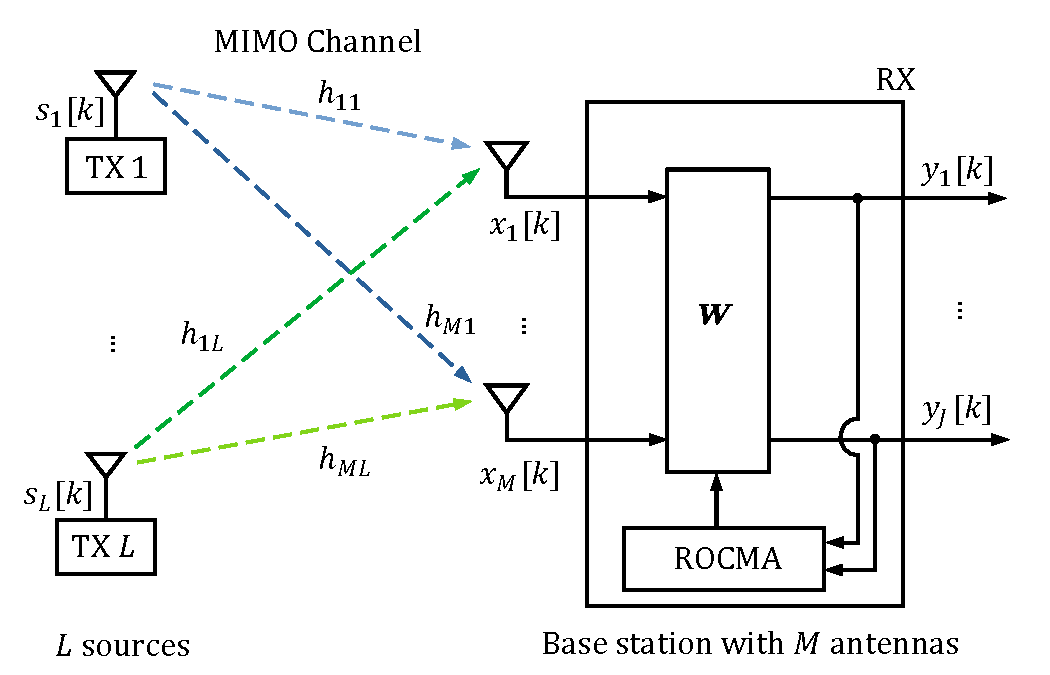
\includegraphics[width=0.6\linewidth]{./figs/rocma_figs/RMSR_system_model_4.pdf}
	\caption{$L$ sources share a common resource block and transmit independent signals to a host station with $M$ antennas through an unknown physical channel. The host receiver aims to find an adaptive linear matrix demixer $\bm{W}$ to recover $J\leq L$ sources with little mutual interference.}\label{rocma:fig:system_model}
\end{figure}

Despite their demonstrated successes, regularization approaches exhibit some drawbacks. 
First, the regularizing term typically requires to tune a scalar weight, e.g. $\gamma_0$ in Eq.(\ref{wfcma:eqn:cma_msr}), often by trial and error, and there is no performance guarantee under various possible scenarios.
Second, different regularization approaches might lead to different solutions and performance, while no solution is consistently better than others. 
Additionally, regularizing terms often increase the computation complexity as regularized cost functions would either require additional computations or delicate non-convex optimization steps. 
Finally, regularizing terms proposed in the literature generally are limited to promote pairwise signal orthogonality instead of multi-lateral signal orthogonality, and also require more data samples to successfully suppress mutual interference.

%In our approach based on Riemann geometry, we enforce signal orthogonality among demixer outputs by directly restricting the solution space.
Therefore, we now reformulate the multiple signal recovery problem and enforce signal orthogonality among demixer outputs by directly restricting the solution space.
Recall the definition of $\bm{W}$ as joint demixer matrix in Section~\ref{system:ssec:blind_recovery}. 
Owing to the phase invariance of the CM cost function, the optimum solution satisfies $\hat{\bm{W}}\herm\bm{H}=\bm{P}$ where $\bm{P}\in\mathbb{C}^{J\times L}$ a generalized permutation matrix whose non-zero entries are
all of the form $e^{j\phi}$ instead of being restricted to 1. 
As a result, at the optimum solution we have $\bm{P}\bm{P}\herm=\bm{I}$, with $\bm{I}$ the identity matrix of appropriate size.
We therefore write the joint signal recovery constraint as
\begin{align}
\hat{\bm{W}}\herm\bm{H}\bm{H}\herm\hat{\bm{W}} &=\bm{I}.
\end{align}

However, the BS has no knowledge of the channel $\bm{H}$. 
Therefore, we can leverage source signal orthogonality and white noise property to estimate $\bm{H}\bm{H}\herm$ from the sample covariance matrix of the received data vectors $\bm{x}_k$ (\ref{system:eqn:rxsignal}):
\begin{align}
\bm{R}_{\bm{X}} &= \frac{1}{K}\sum_{k=1}^K \bm{x}_k\bm{x}_k\herm 
\xrightarrow{K\to\infty} \mathbb{E}\{\bm{R}_{\bm{X}}\}= \bm{H}\bm{H}\herm + \sigma^2\bm{I}.
\end{align}

Note that, in the absence of noise, the rank of matrix $\bm{H}\bm{H}\herm\in\mathbb{C}^{M\times M}$ is $L$ ($L\leq M$), i.e., 
the rank of $\bm{H}$.
Thus, we formulate the optimization problem for multiple signal recovery as orthogonal constant modulus algorithm ({\bf OCMA}):
\begin{subequations}
\begin{align}
	%\min\quad&f(\bm{W})=\frac{1}{2K}\sum_{k=1}^{K}\big\|\ddiag(\bm{W}\herm\bm{X}_k\bm{W})-R_2\bm{I}\big\|_F^2 \label{rocma:eqn:cma_msr_cost}\\
	\min\quad&f(\bm{W})=\frac{1}{2K}\sum_{k=1}^{K}\big\|(\bm{W}\herm\bm{X}_k\bm{W})\circ\bm{I}-R_2\bm{I}\big\|_F^2 \label{rocma:eqn:cma_msr_cost}\\
	\rm{s.t.}\quad& \bm{W}\herm\bm{R}_{\bm{X}}\bm{W}=\bm{I},
	\label{rocma:eqn:cma_msr_restriction}
\end{align}\label{rocma:eqn:cma_msr_restricted}
\end{subequations}
where $\bm{X}_k=\bm{x}_k\bm{x}_k\herm$. Hence, the Euclidean gradient of $f(\bm{W})$ is
\begin{subequations}
\begin{align}
	&\nabla_{\bm{W}}f(\bm{W})=
	%	\frac{1}{K}\sum_{k=1}^K\bm{X}_k\bm{W}\big(\ddiag(\bm{W}\herm\bm{X}_k\bm{W})-R_2\bm{I}\big), 
	\frac{1}{K}\sum_{k=1}^K\bm{X}_k\bm{W}\big((\bm{W}\herm\bm{X}_k\bm{W})\circ\bm{I}-R_2\bm{I}\big),\label{rocma:eqn:rtr_egrad}
\end{align}
and for a matrix $\bm{G}$ of
the same size as $\bm{W}$, the directional derivative of $\nabla_{\bm{W}} f(\bm{W})$ in direction $\bm{G}$ is
\begin{align}\hspace*{-1mm}
	&
	\mathrm{D}\big(\nabla_{\bm{W}}f(\bm{W})\big)[\bm{G}]\nonumber\\
	% \nabla_{\bm{W}|\bm{E}}f(\bm{W})\hspace*{-1mm}
%	&\quad=\hspace*{-1mm}
	%\frac{1}{K}\sum_{k=1}^K\bigg(\bm{X}_k\bm{W} \ddiag(\bm{W}\herm\bm{X}_k\bm{E}+\bm{E}\herm\bm{X}_k\bm{W})
	%	\nonumber\\
	%	&\qquad\qquad+
	%\bm{X}_k\bm{E}\big(\ddiag(\bm{W}\herm\bm{X}_k\bm{W})-R_2\bm{I}\big)
	%\bigg).
	&\qquad=\frac{1}{K}\sum_{k=1}^K\Big(\bm{X}_k\bm{W} \big(\bm{I}\circ(\bm{W}\herm\bm{X}_k\bm{G}+\bm{G}\herm\bm{X}_k\bm{W})\big)
%	\nonumber\\&\qquad\qquad
	+\bm{X}_k\bm{G}\big((\bm{W}\herm\bm{X}_k\bm{W})\circ\bm{I}-R_2\bm{I}\big)
	\Big).\label{rocma:eqn:rtr_ehess}
\end{align} \label{rocma:eqn:cma_msr_gradient_Hessian}
\end{subequations}

\subsection{Estimating the Number of Active Sources for Demixing}\label{rocma:ssec:estimate_sources}
Because of the number of active sources $L$ may vary in practice, the literature has often assumed that $L$ is known. 
However, in grant-free access, such assumption would not be practical, since, at best, we would only be able to limit the maximum number of simultaneous users according to synchronization and slotted scheduling. 
Thus we shall first present an approach to estimate the number of active sources. 

% \textcolor{red}{separate section for estimation of $L$ and its nuances? Add also the robust estimation of $L$ via comparison of norm of approximation error to a certain tolerance, which tells how good the approximation is and if we need to increase $L$}

Given that $\bm{H}$ has rank $L\leq M$, the sample covariance matrix $\bm{R}_{\bm{X}}$ in restriction (\ref{rocma:eqn:cma_msr_restriction}) is not strictly positive definite in the absence of noise.
Thus, (\ref{rocma:eqn:cma_msr_restriction}) cannot be directly defined as a Riemannian manifold. 
In noisy scenarios and with several data samples, the sample covariance matrix will likely be positive definite, but could be numerically ill-conditioned with large condition number. 
However, in both cases we can extract a strictly positive definite matrix from the sample covariance matrix from its rank-$L$ approximation. 

We first estimate the number of transmitted signals embedded in the received data via Minka's Laplace method \cite{Minka2000laplaceTR}, and let the result
be $L$. 
Let the SVD of the channel matrix $\bm{H} = \bm{U}\bm{\Sigma}\bm{V}\herm$, with $\bm{U}\in\mathcal{U}(M)$, and $\bm{V}\in\mathcal{U}(L)$, i.e.,
%After thinking about how to approach this issue, I got an idea: to extract the positive definite portion of the matrix $\bm{R}_{\bm{x}}$ and build a generalized Stiefel manifold from it. 
\begin{align}
	\bm{H}&=[\bm{U}_L\,\,\bm{U}_L^{\perp}]\begin{bmatrix}
		\bm{\Sigma}_L\\\bm{0}_{(M-L)\times L}
	\end{bmatrix}\bm{V}\herm=\bm{U}_L\bm{\Sigma}_L\bm{V}\herm\,,\nonumber\\
	&\bm{U}_L\in\St{M}{L}\,,
	% \nonumber\\&
	\bm{U}_L^{\perp}\in\St{M}{M-L}\,,\nonumber\\
	&\bm{\Sigma}_L=\diag(\sigma_1,\ldots,\sigma_L),  
\end{align}
where $\St{M}{L}=\{\bm{A}\in\mathbb{C}^{M\times L}:\bm{A}\herm\bm{A}=\bm{I}_L\}$ is the complex Stiefel manifold of orthonormal $L$-frames in $\mathbb{C}^M$ \cite{Edelman1999stiefel,Sato2014complexstiefel}.

First, consider the noiseless scenario, i.e. $\bm{R}_{\bm{X}}=\mathbb{E}\{\bm{R}_{\bm{X}}\}$
which equals to
\begin{align}
	\bm{H}\bm{H}\herm=\bm{U}\bm{\Sigma}\bm{\Sigma}\herm\bm{U}\herm=\bm{U}_L\bm{\Sigma}_L\bm{\Sigma}_L\herm\bm{U}_L\herm=\bm{U}_L\bm{\Lambda}\herm\bm{U}_L\herm\,. \label{rocma:eqn:covariance_matrix_decomposition}
\end{align}	
From the above decomposition, we can obtain $\bm{U}$ and $\bm{\Sigma}$, but not $\bm{V}$. 
Also, note that $\bm{\Lambda}=\bm{\Sigma}_L\bm{\Sigma}_L\herm$ is diagonal with strictly positive entries because $\bm{H}$ has full-column rank. Both 
$\bm{U}_L,\bm{U}_L^{\perp}$ are full-column rank.

In the noisy case with infinite samples, we have
\begin{align}
	\bm{H}\bm{H}\herm+\sigma^2\bm{I}&=\bm{U}\bm{\Sigma}\bm{\Sigma}\herm\bm{U}\herm+\sigma^2\bm{I}
%	\nonumber\\&
	=\bm{U}\big(\bm{\Sigma}\bm{\Sigma}\herm+\sigma^2\bm{I}\big)\herm\bm{U}\herm=\bm{U}\bm{\Lambda}_1\bm{U}\herm\,, 
\end{align}	
and we form a diagonal matrix $\bm{\Lambda}$ using the $L$ largest diagonal components of $\bm{\Lambda}_1-\sigma^2\bm{I}$, corresponding to eigenvector matrix $\bm{U}_L$. 
We further define $\bm{\Sigma}_L=\bm{\Lambda}^{1/2}$. 
Note that $\sigma^2$ can be estimated by, e.g., averaging the $M-L$ smallest diagonal elements of $\bm{\Lambda}_1$. 
This approach is very similar to the so-called probabilistic PCA  \cite{VidalGPCA2016}, which obtains the principal components of data and a generative model.
However, even though Minka's Laplace method is known for satisfactory performance in the limited sample regime, it relies on the assumption of Gaussian signals and 
could introduce bias when estimating the number of discrete sources. 

Nevertheless, all independent sources contribute with a significant component of the sample covariance matrix, related to its significant eigenvalues, whereas noise will only have minor contributions in other directions as their related eigenvalues are much smaller in high SNR regimes. 
For an under-estimated $L$, the $L$-rank approximation of the sample covariance matrix would likely fail to capture all relevant directions of the channel, leading to mutual signal interference in signal recovery. 
Therefore, we compute the normalized $L$-rank approximation error 
\begin{align}
	\frac{\big\|\bm{R}_{\bm{X}}-\bm{U}_L\bm{\Lambda}\bm{U}_L\herm\big\|}{\|\bm{R}_{\bm{X}}\|}
\end{align}
for comparison against a preset threshold $\epsilon_r$ to decide whether $L$ needs to be increased in a update. 
We also update the $L$-rank approximation of the sample covariance matrix. 
Our test results to be shown later demonstrate the general reliability of this rank estimation method for demixing. 

\section{A Riemannian Manifold Optimization Framework for CMA} \label{rocma:RGD}

The Riemannian framework for optimization on manifolds \cite{Absil2008book} has gained a lot of attention owing to its capability to handle problems
with a real-valued objective function defined on a constrained space,
\begin{equation}
	\underset{\bm{M}\in\mathbb{C}^{m\times n}}{\text{minimize}}\quad f({\bm{M}})\quad\text{s.t.}\quad\bm{M}\in\mathcal{M}.
\end{equation} 

Note that the (nonlinear) space $\mathcal{M}$ may not be well-defined in terms of addition, continuity, and/or other properties that are typically exploited by regular 
optimization approaches in Euclidean spaces. 
The main idea is to redefine a constrained optimization in Euclidean space
into an unconstrained optimization problem over a manifold. 
Manifolds are topological spaces that, equipped with a metric, locally resemble 
Euclidean spaces of equal dimension size, but may be quite different globally.
%Manifolds are topological spaces that locally resemble Euclidean space of the same dimensionality near each point. In particular, a smooth manifold is defined as a set $\bm{M}$ that locally resembles Euclidean space of the same dimensionality, but can be very different in global terms, where the smoothness plays a key role in the application of classical optimization procedures. 
Some manifold examples include spheres, the set of rotations, the set of positive semidefinite matrices, the set of fixed-rank matrices, and Stiefel manifolds, among many others. 

In this section, we first obtain a suitable Riemannian manifold representation of the CMA problem with orthogonality constraints (\ref{rocma:eqn:cma_msr_restricted}), which we denote Riemannian Orthogonal CMA, or ROCMA.
Next, we further exploit the obtained Riemannian manifold to define a 
quotient Riemannian manifold, with which we can
tackle the phase invariance of the demixers directly in the optimization process.

\subsection{Redefining the Geometry of Signal Recovery}
Our goal here is to find a suitable geometry that encodes the orthogonality condition of demixers in the search space of Problem (\ref{rocma:eqn:cma_msr_restricted}). 
Even with a method to estimate the number of sources $L$, we derive a general version of the geometry where the receiver attempts to recover $J\leq L$ sources. 
Considering Eq.(\ref{rocma:eqn:covariance_matrix_decomposition}) in restriction (\ref{rocma:eqn:cma_msr_restriction}), we have
\begin{align}
	\bm{I}_{J}&=\hat{\bm{W}}\herm\bm{H}\bm{H}\herm\hat{\bm{W}}= \hat{\bm{W}}\herm\bm{U}_L\bm{\Sigma}_L\bm{\Sigma}_L\herm\bm{U}_L\herm\hat{\bm{W}}.\label{rocma:eqn:restriction_svd}
	%\nonumber\\
	%&=\big(\bm{U}_L\herm\hat{\bm{W}}\big)\herm\bm{\Lambda}\big(\bm{U}_L\herm\hat{\bm{W}}\big)
	%=\bm{Y}\herm\bm{\Lambda}\bm{Y}\,,
\end{align}

By introducing a new variable $\bm{Y}$ such that %$\bm{W}=\bm{U}_L\bm{\Sigma}_L^{-1}\bm{Y}$
\begin{align}
	\bm{W}=\bm{U}_L\bm{\Sigma}_L^{-1}\bm{Y},\label{rocma:eqn:transform_Y_W}
\end{align}
Eq.(\ref{rocma:eqn:restriction_svd}) yields $\bm{Y}\herm\bm{Y}=\bm{I}_{\ell}$, which defines the complex Stiefel manifold $\St{L}{J}$. 
%Alternatively, the change of variable $\bm{W}=\bm{U}_L\bm{Y}$ defines defines the complex scaled Stiefel manifold of
%\begin{align}
%	\StL{\bm{\Lambda}}{L}{J}=\{\bm{Y}\in\mathbb{C}^{L\times J}: \bm{Y}\herm\bm{\Lambda}\bm{Y}=\bm{I}_{\ell}\},
%\end{align}
%which is the set of orthonormal $J$ frames in $\mathbb{C}^L$ through the scaling of $\bm{\Lambda}$, and is a generalization of the complex Stiefel manifold $\mathrm{ST}{L}{J}$ (see \cite{Edelman1999stiefel} for the notion of scaled Stiefel manifold in the real case).
Hence, by means of the transformation (\ref{rocma:eqn:transform_Y_W}), we obtain a Riemannian manifold representation of restriction (\ref{rocma:eqn:cma_msr_restriction}) as $\overline{\mathcal{M}}=\St{L}{J}$ that we can use for optimization purposes. 
From the solution in terms of $\bm{Y}$, we obtain the demixer matrix directly by a one-to-one scaling by $\bm{U}_L\bm{\Sigma}_L^{-1}$. The variable transformation (\ref{rocma:eqn:transform_Y_W})
implies the need to rewrite the cost function, Euclidean gradient, and directional derivatives of the gradient. 
Defining $\bm{z}_k=\bm{\Sigma}_L^{-1}\bm{U}_L\herm\bm{x}_k$ and $\bm{Z}_k=\bm{z}_k\bm{z}_k\herm=\bm{\Sigma}_L^{-1}\bm{U}_L\herm\bm{X}_k\bm{U}_L\bm{\Sigma}_L^{-1}$, we have a new cost function
\begin{align}
	\overline{\overline{g}}(\bm{Y})
	%	&=\frac{1}{2K}\sum_{k=1}^{K}\big\|\ddiag(\bm{Y}\herm\bm{Z}_k\bm{Y})-R_2\bm{I}\big\|_F^2
	&=\frac{1}{2K}\sum_{k=1}^{K}\big\|(\bm{Y}\herm\bm{Z}_k\bm{Y})\circ\bm{I}-R_2\bm{I}\big\|_F^2
	\,,\label{rocma:eqn:wfcost_Y}	
\end{align}
whose Euclidean gradient is
\begin{align}	\nabla_{\bm{Y}}\overline{\overline{g}}(\bm{Y})&=
	%	\frac{1}{K}\sum_{k=1}^K\bm{Z}_k\bm{Y}\big(\ddiag(\bm{Y}\herm\bm{Z}_k\bm{Y})-R_2\bm{I}\big), 
	\frac{1}{K}\sum_{k=1}^K\bm{Z}_k\bm{Y}\big((\bm{Y}\herm\bm{Z}_k\bm{Y})\circ\bm{I}-R_2\bm{I}\big), 
	\label{rocma:eqn:wf_egrad_Y}
\end{align} 
and the directional derivative of (\ref{rocma:eqn:wf_egrad_Y}) in direction $\bm{G}$ is
\begin{align}
	\mathrm{D}\big(\nabla_{\bm{Y}}\overline{\overline{g}}(\bm{Y})\big)[\bm{G}]
%	=\nonumber\\
	%	&\qquad\frac{1}{K}\sum_{k=1}^K\bm{Z}_k\bm{Y}\ddiag(\bm{Y}\herm\bm{Z}_k\bm{E}+\bm{E}\herm\bm{Z}_k\bm{Y})
	%	\nonumber\\	&\qquad\qquad
	%	+\bm{Z}_k\bm{E}\big(\ddiag(\bm{Y}\herm\bm{Z}_k\bm{Y})-R_2\bm{I}\big).
%	&\qquad
	&=\frac{1}{K}\sum_{k=1}^K\bm{Z}_k\bm{Y}\big((\bm{Y}\herm\bm{Z}_k\bm{G}+\bm{G}\herm\bm{Z}_k\bm{Y})\circ\bm{I}\big)
%	\nonumber\\	&\qquad\qquad
	+\bm{Z}_k\bm{G}\big((\bm{Y}\herm\bm{Z}_k\bm{Y})\circ\bm{I}-R_2\bm{I}\big). \label{rocma:eqn:wf_ehess_Y}	
\end{align}

To optimize $\bm{Y}$ over $\overline{\mathcal{M}}$, we need to first define the linear space that approximates the manifold around a point $\bm{Y}$, which is called the tangent space at $\bm{Y}$ and is denoted as $\mathrm{T}_{\bm{Y}}\overline{\mathcal{M}}$. 
For $\overline{\mathcal{M}}=\St{L}{J}$, the tangent space is
\begin{align}
	\mathrm{T}_{\bm{Y}}\overline{\mathcal{M}}&=\{\bm{E}\in\C^{L\times J}:\bm{E}=\bm{Y}\bm{\Omega}+\bm{Y}_{\perp}\bm{A},
%	\nonumber\\&\quad\qquad
	\,\bm{\Omega}=-\bm{\Omega}\herm\in\C^{J\times J}, \bm{A}\in\C^{(L-J)\times J}\}.
\end{align}
In other words, $\bm{Y}\herm
%\bm{\Lambda}
\bm{E}=\bm{\Omega}$ is skew-Hermitian $\forall\bm{E}\in\mathrm{T}_{\bm{Y}}\overline{\mathcal{M}}$. Its orthogonal complement is known as \emph{normal} space $\mathrm{N}_{\bm{Y}}\overline{\mathcal{M}}$ and it is given by
\begin{align}
	\mathrm{N}_{\bm{Y}}\overline{\mathcal{M}}&=\{\bm{Y}\bm{A},\,\,\bm{A}=\bm{A}\herm\in\C^{J\times J}\}.
\end{align}

We can now define length in the tangent space with a Riemannian metric $d_{\bm{Y}}$, which is a smooth inner product defined at each element $\bm{Y}$ for elements of the tangent space $\mathrm{T}_{\bm{Y}}\overline{\mathcal{M}}$. 
Here, we use the real-trace inner product, given by
\begin{equation}
	d_{\bm{Y}}(\bm{E},\bm{C})=\re\big(\Tr(\bm{E}\herm
	%\bm{\Lambda}
	\bm{C})\big)\,,\quad \bm{E},\bm{C}\in\mathrm{T}_{\bm{Y}}\overline{\mathcal{M}}.
\end{equation} 

We also define a projection to the tangent space, which allows us to restrict optimization only in the directions of interest, which indeed belong to the tangent space. 
For $\bm{G}\in\mathbb{C}^{L\times J}$, the projection operator is
\begin{align}
	\mathrm{Proj}_{\bm{Y}}^{\mathrm{T}}(\bm{G})&=\bm{G}-\bm{Y}\mathrm{herm}\big(\bm{Y}\herm
	%\bm{\Lambda}
	\bm{G}\big)\in\mathrm{T}_{\bm{Y}}\overline{\mathcal{M}}\,,
\end{align}
which enables us to define the Riemannian gradient and Riemannian Hessian from the Euclidean gradient and its directional derivative, respectively.

For optimization purposes, the motion along the manifold from point $\bm{Y}$ in a given direction $\bm{E}$ is given by a retraction $\mathrm{R}_{\bm{Y}}^{\mathrm{St}}(\bm{E})$, which in our case we select as the polar retraction for the complex Stiefel manifold \cite{Edelman1999stiefel}
\begin{align}
	\mathrm{R}_{\bm{Y}}^{\mathrm{St}}(\bm{E})&=(\bm{Y}+\bm{E})\big((\bm{Y}+\bm{E})\herm
	%\bm{\Lambda}
	(\bm{Y}+\bm{E})\big)^{-0.5}
%	\nonumber\\&
	=(\bm{Y}+\bm{E})\big(\bm{I}+\bm{E}\herm
	%\bm{\Lambda}
	\bm{E}\big)^{-0.5}.
\end{align}


\subsection{Riemannian Quotient Geometry}
%Recall that the cost function (\ref{rocma:eqn:cma_msr_cost}) presents phase invariance in each demixer. 
In the context of Riemannian manifold optimization, quotient Riemannian manifolds are used to define a manifold that presents invariance of the cost function or the representation of the manifold itself  \cite{boumal2020intromanifolds}. 
It can be defined by equipping the original or ambient manifold with an equivalence relation between its points to describe the aforementioned invariance. 

Let $\sim$ be such an equivalence relation, i.e., $\bm{Y}\sim\bm{Y}_0$ denotes that $\bm{Y}$ and $\bm{Y}_0$ are equivalent in terms of the invariance of interest. 
Thus, we can identify equivalent points to $\bm{Y}$ as one single set known as equivalence class, denoted as 
\begin{align}
	[\bm{Y}]=\{\bm{Y}_0\in\mathcal{M}: \bm{Y}_0\sim\bm{Y}\}.
\end{align}
When the quotient space of the ambient manifold $\overline{\mathcal{M}}$ under the equivalence relation $\sim$ satisfies certain conditions \cite[Chapter 3]{Absil2008book}, it is a Riemannian quotient manifold, which is the set of equivalence classes:
\begin{align}
	\mathcal{M}=\overline{\mathcal{M}}/\!\sim\,=\big\{[\bm{Y}]:\bm{Y}\in\overline{\mathcal{M}}\big\}.
\end{align}

A quotient manifold is an abstract space whose elements are subsets of the ambient manifold. 
However, the use of quotient manifolds in Riemannian optimization has additional advantages, such as the ability of obtaining a strictly positive definite Hessian by neglecting directions related to the cost function invariance, and potential reduction of problem dimensionality by applying a simple representation of the elements in the space.
Even in a case when there is no such representation and the ambient manifold is used for computational purposes, the quotient geometry is theoretically important to establish convergence properties of second-order methods that rely on the positive definiteness of the Hessian on the manifold.

Now, recall that the cost function (\ref{rocma:eqn:cma_msr_cost}) presents permutation invariance in the demixers, and unimodular phase invariance in each demixer such that for each demixer $\bm{w}_{\ell}$, a rotated demixer $\e{j\theta}\bm{w}_{\ell}, \theta\in[0,2\pi]$ yields the same cost value.  However, the permutation group is discrete, and thus is a Lie group of dimension 0. This means that in terms of local behavior, the equivalence classes of permutations behaves exactly the same as the ambient manifold, and thus we dismiss the permutations in our analysis and focus exclusively in the phase invariance.

When considering multiple demixers in $\bm{W}$, we want to describe unimodular phase invariance on each of the $J$ demixers simultaneously. 
Let $\mathcal{U}(1)^{\times J}$ be the group of diagonal unitary matrices of size $J$, i.e.
\[\mathcal{U}(1)^{\times J} =\Big\{\bm{D}\in\mathcal{U}(J):\bm{D}=\diag\big(\e{j\theta_1}\,\,\cdots\,\,\e{j\theta_{J}}\big)\,,\,\theta_{\ell}\in[0,2\pi)\,\forall \ell\in\{1,\cdots,J\}\Big\}.\]

Thus, the group action of $\mathcal{U}(1)^{\times J}$ defines an equivalence relation between demixer matrices. 
The corresponding equivalence class is then
\begin{align}
	[\bm{W}]=\big\{\bm{W}\bm{D}:\bm{D}\in\mathcal{U}(1)^{\times J}\big\},\nonumber
\end{align}
and by means of (\ref{rocma:eqn:transform_Y_W}), we have that $\bm{W}\bm{D}=\bm{U}_L\bm{\Sigma}_L^{-1}\bm{Y}\bm{D}$, i.e. the equivalence class in terms of $\bm{Y}$ is 
\begin{align}
	[\bm{Y}]=\big\{\bm{Y}\bm{D}:\bm{D}\in\mathcal{U}(1)^{\times J}\big\}, \label{rocma:eqn:equivalenceclass}
\end{align}
and we obtain a quotient space that considers the cost function invariance as
\begin{align}
	\mathcal{M}= \overline{\mathcal{M}}/\mathcal{U}(1)^{\times J}
\end{align}
with a canonical projection $\pi:\overline{\mathcal{M}}\to\mathcal{M}:\bm{Y}\mapsto[\bm{Y}]$.

Furthermore, $\mathcal{M}$ is indeed a Riemannian quotient manifold (which ensures $\pi$ is smooth). This follows from the fact that the group action of diagonal unitary matrices is smooth, free and proper \cite[Section 9.2]{boumal2020intromanifolds}: (a) it is smooth because it is a matrix multiplication; (b) it is free because $\bm{Y}\bm{D}=\bm{Y}$ implies $\bm{D}=\bm{I}$ by left multiplication of $\bm{Y}\herm$; and (c) it is proper because $\mathcal{U}(1)^{\times J}$ is the maximal torus of the unitary group (a compact group), and thus is compact. Hence, the equivalence classes all have dimension $J$ and are closed embedded submanifolds of $\mathcal{M}$. This quotient manifold has been introduced before in the context of subspace estimation \cite{Palka2015}, but to the best of our knowledge it has not been developed or used in Riemannian optimization.

The quotient manifold $\mathcal{M}$ is an abstract space, and requires matrix representations in the computational space $\overline{\mathcal{M}}$. 
Fortunately, an (abstract) element ${\bm{Y}}_q$ on the quotient manifold can be represented by an element $\bm{Y}$ in the computational space.
Thus, every geometry-related operation over the quotient manifold can be defined in terms of elements and operations in the computational space. 

% \textcolor{red}{clarify lifting and link with quotient manifold and Vy, Hy}
%itemization might help with this dense paragraph. Highlight to what spaces Vy and Hy belong to. 
In particular, we look for a representation of the tangent space of the quotient manifold $\mathrm{T}_{\bm{Y}}\mathcal{M}$ using tangent vectors of the ambient manifold $\overline{\mathcal{M}}$. 
We accomplish this by characterizing the tangent space $\mathrm{T}_{\bm{Y}}\overline{\mathcal{M}}$ as the direct sum of two orthogonal spaces: the \textit{vertical} space $\mathrm{V}_{\bm{Y}}$, which contains the directions tangent to the equivalence classes, and the \textit{horizontal} space $\mathrm{H}_{\bm{Y}}$, which contains the tangent directions orthogonal to the vertical space. 
That is, the horizontal space contains the directions of interest in terms of optimization. Hence, an (abstract) tangent vector of the quotient manifold $\bm{\eta}_{[\bm{Y}]}$ can be represented as an horizontal vector $\bm{\eta}_{\mathrm{H}_{\bm{Y}}}$ of the ambient manifold, which is called the \emph{horizontal lift}, defined as $\bm{\eta}_{\mathrm{H}_{\bm{Y}}}=\mathrm{lift}_{\bm{Y}}(\bm{\eta}_{[\bm{Y}]})$. When $\mathcal{M}$ is endowed with the Riemannian metric inherited from $\overline{\mathcal{M}}$,
\begin{align}
	d_{[\bm{Y}]}(\bm{\eta},\bm{\xi})=d_{\bm{Y}}\big(\mathrm{lift}_{\bm{Y}}(\bm{\eta}),\mathrm{lift}_{\bm{Y}}(\bm{\xi})\big)\,,\,\, \bm{\eta},\bm{\xi}\in\mathrm{T}_{[\bm{Y}]}{\mathcal{M}},\nonumber
\end{align}
the canonical projection $\pi$ forms a Riemannian submersion from the quotient manifold to the computational space, thereby defining a correspondence between elements of $\mathcal{M}$ and elements of $\overline{\mathcal{M}}$ \cite{Absil2008book}. 
Figure~\ref{rocma:fig:qmanifold} shows a depiction of the quotient manifold geometry and its relation to the ambient manifold.
\begin{figure}
	\centering
	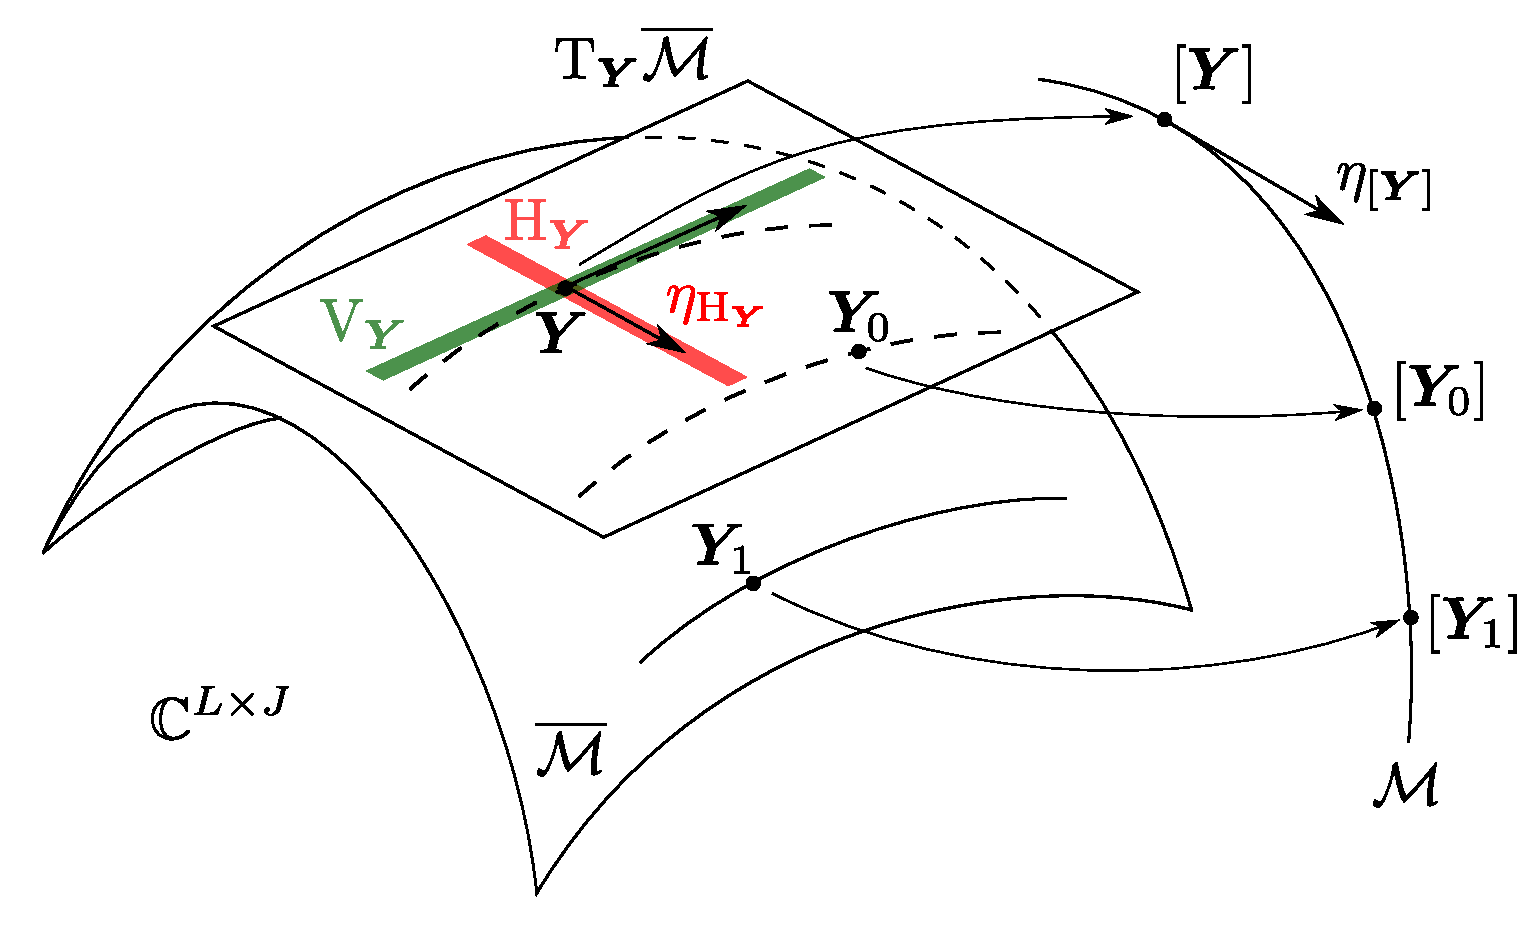
\includegraphics[width=0.65\linewidth]{./figs/rocma_figs/q_manifold_8.pdf}
	\caption[Representation of the ambient manifold and quotient manifold.]{Representation of the ambient manifold $\overline{\mathcal{M}}$ and quotient manifold $\mathcal{M}$. The tangent space $\mathrm{T}_{\bm{Y}}\overline{\mathcal{M}}$ is divided into a vertical space $\mathrm{V}_{\bm{Y}}$ (in green) and a horizontal space $\mathrm{H}_{\bm{Y}}$ (in red), which contains the relevant search directions $\eta_{\mathrm{H}_{\bm{Y}}}$. These directions correspond to  tangent directions $\eta_{[\bm{Y}]}$ at the point $[\bm{Y}]$ in the quotient manifold.}\label{rocma:fig:qmanifold}
\end{figure}

We now define the vertical and horizontal spaces. Let $\bm{D}:\mathbb{R}\to\mathcal{U}(1)^{\times J}$ be a path in the equivalence class such that $\bm{D}(0)=\bm{I}$. 
The vertical space is given by vectors of the form $\bm{YD}'(0)$ where vectors $\bm{D}'(t)$ are tangent to $\mathcal{U}(1)^{\times J}$, whose tangent set corresponds to the Lie algebra of unitary diagonal matrices $\bm{\mathfrak{t}}(J)$, consisting of diagonal imaginary matrices of size 
$J\times J$. 
Therefore, 
\begin{align}
	\mathrm{V}_{\bm{Y}}&=\big\{\bm{YT}:\bm{T}\in\bm{\mathfrak{t}}(J)\big\}
%	\nonumber\\&
	=\{\bm{YT}:\bm{T}\in\mathbb{C}^{J \times J}\text{ diagonal imaginary}\},
\end{align}
and the horizontal space is then given by
\begin{align}
	\mathrm{H}_{\bm{Y}}=\big(\mathrm{V}_{\bm{Y}}\big)^{\perp}
%	\nonumber\\
	&=\{\bm{E}\in\mathrm{T}_{\bm{Y}}\mathcal{M}:\langle \bm{E},\bm{F}\rangle=0\quad\forall\bm{F}\in\mathrm{V}_{\bm{Y}}\}\nonumber\\
	&=\{\bm{E}\in\mathrm{T}_{\bm{Y}}\mathcal{M}:\langle \bm{E},\bm{YT}\rangle=0\quad\forall\bm{T}\in\bm{\mathfrak{t}}(J)\}\nonumber\\
	&=\{\bm{E}\in\mathrm{T}_{\bm{Y}}\mathcal{M}: \re\big(\Tr(\bm{E}\herm
	%\bm{\Lambda}
	\bm{ YT})\big)=0\quad\forall\bm{T}\in\bm{\mathfrak{t}}(J)\}
\end{align}
and thus $\bm{Y}\herm
%\bm{\Lambda}
\bm{E}$ is skew-Hermitian with zero diagonal, to be orthogonal to any $\bm{T}\in\mathfrak{t}(J)$. 
This is equivalent to state that the projection to horizontal space is given by
\begin{align}
	\mathrm{Proj}_{\bm{Y}}^{\mathrm{H}}(\bm{G})
	&=\mathrm{Proj}_{\bm{Y}}^{\mathrm{T}}(\bm{G})
	%-\bm{Y}\ddiag\big(\bm{Y}\herm
	-\bm{Y}\Big(\bm{I}\circ\big(\bm{Y}\herm
	%\bm{\Lambda}
	\mathrm{Proj}_{\bm{Y}}^{\mathrm{T}}(\bm{G})\big)\Big)\nonumber\\
%	&\qquad
	&=\bm{G}-\bm{Y}\mathrm{herm}\big(\bm{Y}\herm
	%\bm{\Lambda}
	\bm{G}\big)
	%\nonumber\\
	%&\quad
	%-\bm{Y}\ddiag\big(\mathrm{skew}(\bm{Y}\herm
	-\bm{Y}\big(\bm{I}\circ\mathrm{skew}(\bm{Y}\herm
	%\bm{\Lambda}
	\bm{G})\big).
	%\nonumber\\
	%&=\bm{E}-\bm{Y}\mathrm{herm}\big(\bm{Y}\herm\bm{\Lambda}\bm{E}\big)-j\bm{Y}\im\ddiag(\bm{Y}\herm\bm{\Lambda E}).
\end{align}

Finally, we can inherit the retraction from the ambient manifold via lifting and enforcing the equivalence class. Indeed, for $\bm{E}=\mathrm{lift}_{\bm{Y}}(\bm{\eta})$, we can see that the polar retraction depends only on the equivalence class:
\begin{align}
	\mathrm{R}_{[\bm{Y}]}(\bm{\eta})&=\mathrm{R}_{\bm{YD}}^{\mathrm{St}}(\bm{E})
%	\nonumber\\&
	=(\bm{YD}+\bm{ED})\big(\bm{I}+(\bm{ED})\herm
	%\bm{\Lambda}
	\bm{ED}\big)^{-0.5}
%	\nonumber\\&
	=\mathrm{R}_{\bm{Y}}^{\mathrm{St}}(\bm{E})\bm{D}=\big[\mathrm{R}_{\bm{Y}}^{\mathrm{St}}(\bm{E})\big].
\end{align}

Consequently, we can effectively optimize over the quotient manifold $\mathcal{M}$ using representatives from the ambient manifold $\overline{\mathcal{M}}$. Moreover, as $\overline{\mathcal{M}}$ is an embedded submanifold of Euclidean space, we can obtain the Riemannian gradient and Hessian in terms of objects in Euclidean space, which is convenient as we already know the cost function $\overline{\overline{g}}$ in Euclidean space given by (\ref{rocma:eqn:wfcost_Y}) with corresponding derivatives (\ref{rocma:eqn:wf_egrad_Y}) and (\ref{rocma:eqn:wf_ehess_Y}). We denote $\overline{g}=\overline{\overline{g}}\big|_{\overline{\mathcal{M}}}$ the restriction of the Euclidean cost function to the ambient manifold. As $\overline{g}$ is invariant under $\sim$, the cost function $g$ defined in $\mathcal{M}$ is smooth and $g([\bm{Y}])=\overline{g}(\bm{Y})$. Hence, by definition, the Riemannian gradient of $g$ is zero for vertical vectors (as they are invariance directions), and we have
\begin{align}
	&\mathrm{lift}_{\bm{Y}}\big(\gradh g([\bm{Y}])\big)
	=\grad \overline{g}(\bm{Y})
%	\nonumber\\&\quad
	=\mathrm{Proj}_{\bm{Y}}^{\mathrm{H}}\big(\nabla_{\bm{Y}} \overline{\overline{g}}(\bm{Y})\big) 
	% 	\nonumber\\&
	= \mathrm{Proj}_{\bm{Y}}^{\mathrm{T}}\big(\nabla_{\bm{Y}} \overline{\overline{g}}(\bm{Y})\big), \label{rocma:eqn:lifted_grad}
\end{align}
where we can choose the most convenient projection to obtain the lifted gradient, thus we use the projection to tangent space:
\begin{align}
	&\mathrm{lift}_{\bm{Y}}\big(\gradh g ([\bm{Y}]\big) = \mathrm{Proj}_{\bm{Y}}^{\mathrm{T}}\big(\nabla_{\bm{Y}} \overline{\overline{g}}(\bm{Y})\big)
%	\nonumber\\&\quad
	= \nabla_{\bm{Y}} \overline{\overline{g}}(\bm{Y})-\bm{Y}\mathrm{herm}\big(\bm{Y}\herm\nabla_{\bm{Y}} \overline{\overline{g}}(\bm{Y})\big)\nonumber\\
	&\quad= \frac{1}{K}\sum_{k=1}^K\bm{Z}_k\bm{Y}\big((\bm{Y}\herm\bm{Z}_k\bm{Y})\circ\bm{I}-R_2\bm{I}\big)
%	\nonumber\\&\qquad\qquad
	-\bm{Y}\mathrm{herm}\big(\bm{Y}\herm\bm{Z}_k\bm{Y}\big((\bm{Y}\herm\bm{Z}_k\bm{Y})\circ\bm{I}-R_2\bm{I}\big)\big).\label{rocma:eqn:lifted_grad_derived}
\end{align}

The horizontal lift of the Riemannian Hessian of $g$ in terms of $\overline{\overline{g}}$ is given by
\begin{align}
	\mathrm{lift}_{\bm{Y}}\big(\Hessh g([\bm{Y}])[\bm{\eta}]\big)
	&=\mathrm{Proj}_{\bm{Y}}^{\mathrm{H}}\big(\Hess \overline{{g}}(\bm{Y})[\bm{E}]\big)
%	\nonumber\\&= 
	\mathrm{Proj}_{\bm{Y}}^{\mathrm{H}}\big(\mathrm{D} \overline{\overline{r}}(\bm{Y})[\bm{E}]\big),\label{rocma:eqn:lifted_hess}
\end{align}
with $\bm{E}=\mathrm{lift}_{\bm{Y}}(\bm{\eta})$ and $\overline{\overline{r}}$ a smooth extension of $\grad\overline{g}$ to a neighborhood of $\overline{\mathcal{M}}$ in Euclidean space $\mathbb{C}^{L\times J}$. An obvious choice is 
\begin{align}
	\overline{\overline{r}}(\bm{Y}) &= \nabla_{\bm{Y}} \overline{\overline{g}}(\bm{Y})-\bm{Y}\mathrm{herm}\big(\bm{Y}\herm\nabla_{\bm{Y}} \overline{\overline{g}}(\bm{Y})\big)\nonumber\\ &=\frac{1}{K}\sum_{k=1}^K\bm{Z}_k\bm{Y}\big((\bm{Y}\herm\bm{Z}_k\bm{Y})\circ\bm{I}-R_2\bm{I}\big)
%	\nonumber\\&\qquad\quad
	-\bm{Y}\mathrm{herm}\big(\bm{Y}\herm\bm{Z}_k\bm{Y}\big((\bm{Y}\herm\bm{Z}_k\bm{Y})\circ\bm{I}-R_2\bm{I}\big)\big),\nonumber
\end{align}
with directional derivatives
\begin{align}
	\mathrm{D}\overline{\overline{r}}(\bm{Y})[\bm{G}] &= \mathrm{D}\big(\nabla_{\bm{Y}}\overline{\overline{g}}(\bm{Y})\big)[\bm{G}]
	-\bm{G}\mathrm{herm}\big(\bm{Y}\herm\nabla_{\bm{Y}} \overline{\overline{g}}(\bm{Y})\big)
%	\nonumber\\&\qquad
	-\bm{Y}\mathrm{herm}\big(\mathrm{D}\big(\bm{Y}\herm\nabla_{\bm{Y}} \overline{\overline{g}}(\bm{Y})\big)[\bm{G}]\big),\nonumber
\end{align}
and the lifted Riemannian Hessian is
\begin{align}
	&\mathrm{lift}_{\bm{Y}}\big(\Hessh g \big([\bm{Y}]\big)[\bm{\eta}]\big)
	% 	= \mathrm{Proj}_{\bm{Y}}^{\mathrm{H}}\Big(\mathrm{D}\overline{\overline{r}}(\bm{Y})[\bm{E}]\Big)
	\nonumber\\
	&\qquad=\mathrm{Proj}_{\bm{Y}}^{\mathrm{H}}\Big(\mathrm{D}\big(\nabla_{\bm{Y}}\overline{\overline{g}}(\bm{Y})\big)[\bm{E}]
	-\bm{E}\mathrm{herm}\big(\bm{Y}\herm\nabla_{\bm{Y}} \overline{\overline{g}}(\bm{Y})\big)
%	\nonumber\\&\qquad\qquad\quad
	-\bm{Y}\mathrm{herm}\big(\mathrm{D}\big(\bm{Y}\herm\nabla_{\bm{Y}} \overline{\overline{g}}(\bm{Y})\big)[\bm{E}]\big)\Big)
	\nonumber\\
	&\qquad=\mathrm{Proj}_{\bm{Y}}^{\mathrm{H}}\Big(\mathrm{D}\big(\nabla_{\bm{Y}}\overline{\overline{g}}(\bm{Y})\big)[\bm{E}]
	-\bm{E}\mathrm{herm}\big(\bm{Y}\herm\nabla_{\bm{Y}} \overline{\overline{g}}(\bm{Y})\big)\Big),\label{rocma:eqn:lifted_hess_derived}
	%	\nonumber\\
	%	&\qquad=
\end{align}
where the last term of the first equality vanishes through the horizontal projection, because the term belongs to the normal space and $\mathrm{H}_{\bm{Y}}\subset\mathrm{T}_{\bm{Y}}\overline{\mathcal{M}}\perp\mathrm{N}_{\bm{Y}}\overline{\mathcal{M}}$.

Table~\ref{rocma:table:riemmann} summarizes the geometric definitions of the quotient manifold $\mathcal{M}$ (using representatives in $\overline{\mathcal{M}}$) for ROCMA. Readers interested in additional details of the quotient manifold discussions may refer to \cite[Chapter 9]{boumal2020intromanifolds}.

\subsection{Riemannian Optimization for Blind Signal Recovery}

We use a Riemannian Trust-Region (RTR) algorithm, which is a second-order optimization approach with superlinear convergence rate \cite{Absil2007trustregions}. At each iteration, to search a direction $\bm{E}$ in the horizontal space $\mathrm{H}_{\bm{Y}}$ of iterate $\bm{Y}\in\overline{\mathcal{M}}$, RTR solves the trust-region subproblem 
\begin{eqnarray}
	\mathcal{T}:\,\,\underset{\bm{E}\in\mathrm{H}_{\bm{Y}}}{\text{minimize}}\quad& q_{\bm{Y}}(\bm{E})\nonumber\\
	\text{s.t.}\quad&d_{\bm{Y}}(\bm{E},\bm{E})\leq\varepsilon^2
\end{eqnarray}
in the ambient manifold, where $q_{\bm{Y}}$ is a quadratic model of the cost function at $\bm{Y}\in\overline{\mathcal{M}}$, and $\varepsilon$ denotes the trust region radius. The model is given by
\begin{align}
	q_{\bm{Y}}(\bm{E})&=\overline{g}(\bm{Y})+d_{\bm{Y}}\Big(\bm{E},\grad \overline{g}(\bm{Y})\Big) 
%	\nonumber\\&\quad
	+\frac{1}{2}d_{\bm{Y}}\Big(\bm{E},\mathrm{Proj}_{\bm{Y}}^{\mathrm{H}}\big(\Hess \overline{{g}}(\bm{Y})[\bm{E}]\big)\Big),\nonumber
\end{align}
using the horizontal lifts of both Riemannian gradient and Hessian derived in Eqs.(\ref{rocma:eqn:lifted_grad})-(\ref{rocma:eqn:lifted_hess_derived}). In its general formulation, RTR uses a self-adjoint linear operator instead of the Riemannian Hessian for ease of computation, but can obtain a better performance match using the Hessian.

\begin{table*}[tbh]
	\small\centering
	\caption{Riemannian geometry definitions required for manifold optimization of ROCMA.} \label{rocma:table:riemmann}
	\begin{tabular}{l|l}
		Name&Definition\\[.15em]\hline
		Computational space $\overline{\mathcal{M}}$   & $\St{L}{J}$\\
		Quotient space $\mathcal{M}=\overline{\mathcal{M}}/{\sim}$   & $\St{L}{J}/\mathcal{U}(1)^{\times J}$\\
		Horizontal space $\mathrm{H}_{\bm{Y}}$ & $\mathrm{H}_{\bm{Y}}=\{\bm{E}\in\mathrm{T}_{\bm{Y}}\overline{\mathcal{M}}: \re\big(\Tr(\bm{E}\herm
		%\bm{\Lambda}
		\bm{ YT})\big)=0\quad\forall\bm{T}\in\bm{\mathfrak{t}}(J)\}$\\
		Horizontal space projection $\mathrm{Proj}_{\bm{Y}}^{\mathrm{H}}$& $\mathrm{Proj}_{\bm{Y}}^{\mathrm{H}}(\bm{G})=\bm{G}-\bm{Y}\mathrm{herm}\big(\bm{Y}\herm
		%\bm{\Lambda}
		\bm{G}\big)-\bm{Y}\big(\bm{I}\circ\mathrm{skew}(\bm{Y}\herm
		%\bm{\Lambda}
		\bm{G})\big)$ \\
		Riemannian metric $d_{\bm{Y}}$ & $d_{\bm{Y}}(\bm{E},\bm{C})=\re\big(\mathrm{Tr}(\bm{E}\herm
		%\bm{\Lambda}
		\bm{C})\big)$, $\bm{E},\bm{C}\in\mathrm{H}_{\bm{Y}}$\\
		Retraction $\mathrm{R}_{\bm{Y}}^{\mathrm{St}}$ & $\mathrm{R}_{\bm{Y}}^{\mathrm{St}}(\bm{E})=(\bm{Y}+\bm{E})\big(\bm{I}+\bm{E}\herm
		%\bm{\Lambda}
		\bm{E}\big)^{-0.5}$\\
		Riemannian gradient $\gradh g$ & $\mathrm{lift}_{\bm{Y}}\big(\gradh g ([\bm{Y}]\big) =\mathrm{Proj}_{\bm{Y}}^{\mathrm{T}}\big(\nabla_{\bm{Y}}\overline{\overline{g}}(\bm{Y})\big)$\\
		Riemannian Hessian $\Hessh g$ & $\mathrm{lift}_{\bm{Y}}\big(\Hessh g(\bm{Y})[\bm{E}]\big)$\\
		&$\qquad\qquad
		=\mathrm{Proj}_{\bm{Y}}^{\mathrm{H}}\Big(\mathrm{D}\big(\nabla_{\bm{Y}}\overline{\overline{g}}(\bm{Y})\big)[\bm{E}]
		-\bm{E}\mathrm{herm}\big(\bm{Y}\herm\nabla_{\bm{Y}} \overline{\overline{g}}(\bm{Y})\big)\Big)$\\
		% 		$\\
		% 		&$\quad =\mathrm{Proj}_{\bm{Y}}^{\mathrm{H}}\Big(\mathrm{D}\big(\nabla_{\bm{Y}}\overline{\overline{g}}(\bm{Y})\big)[\bm{E}]
		% 		-\bm{E}\mathrm{herm}\big(\bm{Y}\herm\nabla_{\bm{Y}} \overline{\overline{g}}(\bm{Y})\big)
		% 		-\bm{Y}\mathrm{herm}\big(\mathrm{D}\big(\bm{Y}\herm\nabla_{\bm{Y}} \overline{\overline{g}}(\bm{Y})\big)[\bm{E}]\big)
		%         \Big)$\\
	\end{tabular}
\end{table*}

We can now define the ROCMA algorithm as summarized in Algorithm~\ref{rocma:alg:rocma}. 
Succinctly, we first initialize by estimating the number of sources $L$, perform an $L$-rank eigendecomposition that removes noise contribution in eigenvalues, 
and by corroborating that the $L$-rank approximation is close to the sample covariance matrix to adjust $L$ if needed. 
After scaling the data vectors, we define cost function, quotient Riemannian manifold, and geometry operations. 
Thereafter, we determine Riemannian Trust Regions: in each iteration we solve the trust-regions subproblem $\mathcal{T}$ in the horizontal space of the current iterate, obtaining a descent direction $\bm{E}$ in the horizontal space $\mathrm{H}_{\bm{Y}}$, whose magnitude is given by the size of the accepted trust region \cite{Absil2008book}. 
The subsequent solution iterate is computed using the retraction of $\bm{E}$, which brings the result back to the manifold. 
Once the algorithm converges, we compute the demixer matrix by scaling the obtained solution with $\bm{U}_L\bm{\Sigma}_L^{-1}$.
\begin{algorithm}[htb]
	\caption{Riemannian Orthogonal CMA (ROCMA)}
	\label{rocma:alg:rocma}
	\begin{algorithmic}[1]
		\Statex {\textbf{Given: }$\xk\in\mathbb{C}^M,\,k\in\{1,\ldots,K\}$,  trust region radius $\varepsilon$, low-rank approximation tolerance $\epsilon_r$}
		\Statex \textbf{A) Source estimation:} 
		\State Estimate number of independent sources $L$ with Minka's Laplace method
		\State Obtain $L$ largest eigenvalues and corresponding eigenvectors of sample covariance matrix $\bm{R}_{\bm{X}}$ to construct $L$-rank approximation $\bm{R}_{\bm{X}}=\sum_k\bm{x}_k\bm{x}_k\herm\approx\bm{U}_L\bm{\Sigma}_L^2\bm{U}_L\herm$
		\While{$\|\bm{R}_{\bm{X}}-\bm{U}_L\bm{\Sigma}_L^2\bm{U}_L\herm\|>\epsilon_{r}\|\bm{R}_{\bm{X}}\|$}
		\State $L=L+1$
		\State Update $\bm{\Sigma}_L$, $\bm{\Sigma}_L$ and $\bm{U}_L$ with new components
		\EndWhile
		\Statex \textbf{B) Initialization:} 
		\State Define $\bm{z}_k=\bm{\Sigma}_L^{-1}\bm{U}_L\herm\bm{x}_k$ and objective function $g$
		\State Define geometry ingredients of $\mathcal{M}$ with representatives in $\overline{\mathcal{M}}$ according to Table~\ref{rocma:table:riemmann} 
		\Statex \textbf{C) Riemannian Trust Regions:}
		\While{not converged}
		\State Obtain descent direction $\bm{E}_t$ by solving $\mathcal{T}$ in $\mathrm{H}_{\bm{Y}_t}$
		\State $\displaystyle \bm{Y}_{t+1}=\mathrm{R}_{\bm{Y}_t}^{\mathrm{St}}\big(\bm{E}_t\big)$
		\EndWhile
		\State $\bm{W}_{\mathrm{final}}=\bm{U}_L\bm{\Sigma}_L^{-1}\bm{Y}_{\mathrm{final}}$
	\end{algorithmic}
\end{algorithm}

A known algorithm to solve the trust-region subproblem $\mathcal{Q}$ based in a truncated Conjugate Gradient approach is available as Algorithm~11 in \cite[Section 7.3]{Absil2008book}. 
The manifold optimization toolbox Manopt \cite{manopt} implements a variation of this algorithm. We use this open-source toolbox Manopt in our implementation of Algorithm~\ref{rocma:alg:rocma} by leveraging its flexibility for selectable choices of stopping criteria, tolerances, and other parameters.

\section{Convergence and Analysis} \label{rocma:Performance}

\subsection{Convergence Conditions and Properties of CMA} \label{rocma:subs:known_convergence}
The global convergence properties of CMA for a
single PAM or QAM source recovery in 
noiseless scenarios are well known \cite[Chapters 4-7]{Ding2000}. 
The case of SIMO-CMA blind equalizers, also known as fractionally-spaced CMA or CMA-FSE (when applied to blind equalization scenarios), correspond to the case of recovering one transmitted signal in a grant-free scenario. 
The CMA-FSE equalizer has guaranteed global convergence so long
as the channel matrix $H$ has full column rank \cite{LiDing1994cmaglobalconvergencefse}. Additionally, in \cite{Ding1991} the authors show that in the asymptotic regime and under the aforementioned assumptions, for all stable critical points (desirable or not) the only direction of invariance of the CMA cost function corresponds to the 1-dimensional 
manifold of rotations of the combiner, or $\mathcal{U}(1)$ using our notation in this
chapter. This invariance result is exploited in \cite{Kreutz2008trustregionscma} to further establish conditions for convergence of CMA and adapt a Newton method, discarding search directions in the equivalence class of rotations. 

Multi-channel CMA equalizers are an extension of CMA-FSE, where multiple transmitters
simultaneously send independent source signals on a set of shared channels. 
Targeting one source signal, we can apply CMA to update a receiver 
equalizer that recovers the signal with minimal co-channel
multi-user interference and minimum inter-symbol interference (ISI) \cite{Mayrargue1994mimocma,Li1998adaptivemimocma}.
Global convergence of MIMO-CMA equalizers have similar requirements as the case of CMA-FSE equalizers, which in turn is equivalent to have the channel convolution matrix $\bm{H}$ with full column rank.
Thus, channel matrix $\bm{H}$ of full-column rank provides guaranteed global convergence in noiseless scenarios. 
Multiple source recovery as presented here is a special case of the multiple source recovery scheme presented in \cite{Li1998adaptivemimocma} with zero-ISI subchannels. Thus, global convergence is 
also guaranteed under similar conditions.  
The effect of moderate channel noises on CMA has been shown to be mild by
introducing additional
local minima in the vicinity of the global solution 
\cite{zeng1998relationships,zeng1999analysis}. 
Hence, in the following we will always assume that the channel 
matrix $\bm{H}$ has full-column rank. 


However, most of these works focus in the asymptotic behavior of the CMA cost 
function and its geometry. 
Under finite data sample, 
our recent work \cite{Feres2019wfcma} provides the first analysis
for CMA-based source recovery. Our findings in \cite{Feres2019wfcma} show
that despite being non-convex, the CMA cost function is geometrically well-behaved 
in terms of strong convexity and bounded curvature in a neighborhood of the optimal solutions.
The CMA convergence is therefore tractable in the non-asymptotic case. 
% In particular, one of its results is the concentration of measure of the Euclidean Hessian of the CMA function $f$, i.e., the sample Hessian is close to its expectation with high probability for a sufficiently large number of samples $K$ \cite[Lemma 1]{Feres2019wfcma}. Hence, we can use the expectation to approximate the behavior of the sample Hessian. 
In the remainder of this section, we shall utilize some of the recent
results to bound the minimum eigenvalue of the Euclidean Hessian, in order
to provide convergence guarantee for RTR. 
			
\subsection{Known Results in Relation to ROCMA}

Riemannian manifold optimization with different solvers, such as Riemannian Trust-Regions, has well-known convergence guarantees \cite{Absil2007trustregions} over several classical manifolds, such as the Stiefel manifold and the generalized Stiefel manifold, \cite{Edelman1999stiefel}, the Grassmannian manifold \cite{Absil2008book}, and many others. 
These properties also apply to the quotient Riemannian manifolds, as the computational space is still the ambient manifold \cite{Absil2008book}. In particular, Riemannian Trust regions will converge superlinearly \cite{Absil2007trustregions}.

Previous works have analyzed some particular cases of cost functions that are mathematically similar to Eq.(\ref{rocma:eqn:wfcost_Y}). 
These works present scenarios closely related to the constant modulus portion of the OCMA problem, but did not exploit the (scaled) orthogonality of several solutions in the problem geometry. 
In \cite{Theis2009jointdiagonalizationICA} the authors optimize over the Stiefel manifold to maximize the diagonal terms of a matrix quadratic form for joint diagonalization, which is similar to the CMA cost function by setting $R_2=0$. 
Another work \cite{Bendory2018riemannianphaseretrieval} tackles the phase retrieval problem by defining a manifold geometry with the so-called fixed-norms manifold. 

We now adopt and extend existing analysis to investigate the convergence properties
of ROCMA. 

\subsection{Convergence of ROCMA}
We first make slight modifications to simplify analysis. Recall the SVD of the full rank channel matrix $H$ from Section~\ref{rocma:ssec:estimate_sources}. we can rewrite 
\begin{align}
\bm{W}\herm\bm{x}_k=\bm{Y}\herm\bm{z}_k=\bm{Y}\herm\bm{V}\herm\bm{s}_k+\bm{Y}\herm\bm{n}_k=\bm{Q}\herm\bm{s}_k+\breve{\bm{n}}_k,\nonumber 
%\label{rocma:eqn:parameter_space}
\end{align}
where we use $\breve{\bm{n}}_k= \bm{Y}\herm\bm{n}_k$ to denote the
demixer output noise vector. 
Note that here we use
$\bm{Q}=\bm{V}\bm{Y}=\bm{H}\herm\bm{W}\in\mathbb{C}^{L\times J}$ to
denote the matrix of combined (channel plus demixer) parameter vectors. 
This linear variable transformation between $\bm{Q}$ and $\bm{Y}$ is bijective
since $\bm{H}$ is full-column rank and $\bm{V}$ is orthonormal.
Hence, our analysis will equivalently be performed in $\bm{Q}$-space and 
$\bm{Y}$-space. Without loss of generality, we consider
noiseless scenario for ease of exposition.

As $\bm{Q}$ interacts with independent source signals directly, 
it is straightforward to check whether CMA converges to 
a joint demixer of the form $\widehat{\bm{Q}}=\bm{P}\bm{D}$, 
in which $\bm{P}\in\mathbb{C}^{L\times J}$ is a tall permutation matrix, 
and $\bm{D}$ a diagonal unitary matrix. 
Hence, any optimum solution of ROCMA in the quotient manifold $\mathcal{M}=\St{L}{J}/\mathcal{U}(1)^{\times J}$ has to be of the form $[\widehat{\bm{Y}}]=[\bm{V}\herm\bm{P}]$. Equivalently, in the ambient manifold, the horizontal lift of the optimum is $\widehat{\bm{Y}}=\mathrm{lift}_{[\widehat{\bm{Y}}]}([\widehat{\bm{Y}}])$. In the following, we adopt all these representations equivalently.

Recall that the second order moment, fourth order moment, and kurtosis of 
QAM source signals are defined \cite{Ding2000} by
\begin{align}
m_2=\mathbb{E}\{|s[k]|^2\}, \,\, m_4=\mathbb{E}\{|s[k]|^4\}, \,\,\kappa=m_4-2 m_2^2<0.\nonumber
\end{align} 
We note here that for QAM signals, $4m_2^2+3\kappa\geq m_2^2$ holds. 
We now present the two main theorems that ensure convergence guarantees for ROCMA using RTR.
\begin{thm}[Positive Definiteness of Riemannian Hessian]\label{rocma:thm:ROCMA_hess_posdef}
	Consider signal vector $\bm{s}_k\in\mathbb{C}^L$ with i.i.d. elements from a square QAM constellation of size $Q$. Additionally, let the channel matrix $\bm{H}$ be full-column rank.
	Let $[\widehat{\bm{Y}}]$ be a solution of the ROCMA problem on the quotient manifold $\mathcal{M}=\St{L}{J}/\mathcal{U}(1)^{\times J}$. 
	There exist $C_1>0$ and $c_1>0$ %depending only on the QAM constellation size 
	such that, if the number of measurements $K\geq C_1 L$, the Riemannian Hessian of the cost function $g(\cdot)$ in $\mathcal{M}$ is positive definite in the neighborhood of $[\widehat{\bm{Y}}]$	with probability of at least $1 -6\e{-c_1K}$.
	% 	Furthermore, the CMA problem is globally and locally convergent using Riemannian Trust Regions as defined in Algorithm 1.
\end{thm}

\begin{proof}
	% We first prove that the Riemannian Hessian is strictly positive definite in a neighborhood of an optimum. Moreover, 
	We begin our proof from the case of single-source recovery ($J=1$) before
	generalizing to multiple sources $J>1$.
	
	%cost lifting? be specific and change to formal description
	As the cost function is a sample average, we study the expectation of its Hessian and invoke concentration of measure to approximate the behavior of the Hessian with that of its mean with high probability.
	Let $\widehat{\bm{Q}}\in\mathbb{C}^L$ be an ROCMA minimum in combined parameter space.
	Specifically, $\widehat{\bm{Q}}=\e{j\theta}\bm{e}_{i}$ which denotes arbitrary
	$\theta$ rotation of a canonical vector $\bm{e}_{i}$.
	Invoking \cite[Lemma 1]{Feres2019wfcma}, for $\delta>0$ there exist $C_1(\delta)>0$ and $c_1(\delta)>0$ such that for $K\geq C_1(\delta)L$, the single-source sample Euclidean Hessian is concentrated around its mean, i.e., $\big\|\nabla^2 \overline{\overline{g}}(\widehat{\bm{Q}})-\mathbb{E}\big\{\nabla^2 \overline{\overline{g}}(\widehat{\bm{Q}})\}\big\|\leq\delta$ with probability at least $1-6\e{-c_1(\delta)K}$.
	
	%\textcolor{red}{u nonzero, not necessarily norm1 unless we want to}
	Let $\bm{U}\in\mathbb{C}^L$ a nonzero vector
%	.
	, and let $\tilde{\bm{U}}=[\bm{U}\T\;\bm{U}\herm]\T$. %such that $\|\bm{u}\|=1$.
	% , and let $B(\bm{u},\bm{A})$ be the quadratic form of matrix $\bm{A}$ at $\bm{u}$ using Wirtinger coordinates \cite{Kreutz2008trustregionscma}
	From \cite{Feres2021WFCMA}, 
	the quadratic form of the mean single-source Euclidean Hessian at $\widehat{\bm{Q}}$ (using Wirtinger derivatives as in \cite{Kreutz2008trustregionscma}) is
	\begin{align}
		&\frac{1}{2}
		\tilde{\bm{U}}
%		\begin{bmatrix}
%			\bm{U}\\%[0.2em]
%			\overline{\bm{U}}
%		\end{bmatrix}
		\herm
		\mathbb{E}\big\{\nabla^2 \overline{\overline{g}}(\widehat{\bm{Q}})\big\}
		\tilde{\bm{U}}
%		\begin{bmatrix}
%			\bm{U}\\%[0.2em]
%			\overline{\bm{U}}
%		\end{bmatrix}	
	\nonumber\\&\quad
		= (2m_2^2-R_2m_2)\|\bm{U}\|^2 +(3m_2^2+2\kappa)\re(\bm{U}\herm\widehat{\bm{Q}})^2
%		\nonumber\\&\qquad
		-m_2^2\im(\bm{U}\herm\widehat{\bm{Q}})^2+ (m_2^2+\kappa)|\bm{U}\herm\widehat{\bm{Q}}|^2\nonumber\\
		&\quad= |\kappa|\cdot\|\bm{U}\|^2 +(4m_2^2+3\kappa)\re(\bm{U}\herm\widehat{\bm{Q}})^2
		%	\nonumber\\&\qquad
		+\kappa\im(\bm{U}\herm\widehat{\bm{Q}})^2.\label{rocma:eqn:expectation_euclidean_hessian}
		%\label{rocma:eqn:cor1_lower_bound_1}
	\end{align}

	
	Additionally, knowing that $4m_2^2+3\kappa\geq m_2^2$ and
	\begin{align}
		\im(\bm{U}\herm\widehat{\bm{Q}})^2 \leq \max |U_{i}|^2 \leq \sum_{i=1}^L|U_{i}|^2=\|\bm{U}\|^2, 
	\end{align}
	we see that $\bm{U}$ is a zero solution of Eq.(\ref{rocma:eqn:expectation_euclidean_hessian}) if and only if $\bm{U}$ has one nonzero element corresponding to the nonzero element of $\widehat{\bm{Q}}$, and $\bm{U}\herm\bm{Q}$ is purely imaginary, i.e. $\|\bm{U}\|^2=\im(\bm{U}\herm\widehat{\bm{Q}})^2$. 
	Let $\widehat{\bm{Y}}\in\overline{\mathcal{M}}=\St{L}{1}$ be the horizontal lift of the optimum $[\widehat{\bm{Y}}]$. 
	Recall that
	$\widehat{\bm{Y}}^H \widehat{\bm{Y}}=1$. 
	% , and by definition $\|\widehat{\bm{Y}}\|=1$. 
	From the relationship between $\overline{\mathcal{M}}$ and combined parameter space, i.e. $\bm{Q}=\bm{V}\bm{Y}$ with the matrix $\bm{V}$ formed by right singular vectors of $\bm{H}$, we have that the optimum in combined parameter space is  $\widehat{\bm{Q}}=\bm{V}\widehat{\bm{Y}}$.
	Now let $\bm{G}=\bm{V}\herm\bm{U}$, which we decompose in three orthogonal components: a vertical direction $\bm{E}=\widehat{\bm{Y}}\bm{T}\in\mathrm{V}_{\widehat{\bm{Y}}}$ with $\bm{T}$ imaginary diagonal (i.e., a scalar), a horizontal direction $\bm{F}\in\mathrm{H}_{\widehat{\bm{Y}}}$ and a normal direction $\bm{C}=\widehat{\bm{Y}}\bm{A}\in\mathrm{N}_{\widehat{\bm{Y}}}\overline{\mathcal{M}}$, where $\bm{A}$ is Hermitian (i.e., a real scalar). Hence,
	\begin{align}
		\bm{U}\herm\widehat{\bm{Q}}&=\bm{G}\herm\widehat{\bm{Y}}=\bm{E}\herm\widehat{\bm{Y}}+\bm{F}\herm\widehat{\bm{Y}}+\bm{C}\herm\widehat{\bm{Y}}
		% \nonumber\\&
		=\bm{T}\herm+\bm{A},
	\end{align}
	where we use that $\bm{F}\herm\widehat{\bm{Y}}=0$ because it is skew-Hermitian with zero diagonal and a scalar. Now, given $\bm{U}$ for which $\bm{U}\herm\widehat{\bm{Q}}$ is purely imaginary, the
	Hermitian $\bm{A}$ must be $0$. In conclusion, the \emph{only} directions in the nullspace of the Euclidean Hessian at $\widehat{\bm{Q}}$ in combined parameter space correspond only to vertical directions at $\widehat{\bm{Y}}$ in $\bm{Y}$-space, i.e., $\mathrm{V}_{\widehat{\bm{Y}}}$ corresponds to the nullspace of the Hessian. Therefore, in the quotient manifold $\mathcal{M}$, where the vertical 
	directions are eliminated, the mean Hessian must be positive definite on the manifold. 
					

	Now, according to \cite[Lemma~1]{Feres2019wfcma}, $K>C_1(\delta)L$ implies that $\nabla^2 \overline{\overline{g}}(\widehat{\bm{Q}})\succeq\mathbb{E}\{\nabla^2 \overline{\overline{g}}(\widehat{\bm{Q}})\}-\delta\bm{I}$ with probability of at least $1-6\e{-c_1K}$. 
	From Eq.(\ref{rocma:eqn:expectation_euclidean_hessian})
	we have
	\begin{align}
		\frac{1}{2}
		\tilde{\bm{U}}
%		\begin{bmatrix}
%			\bm{U}\\%[0.2em]
%			\overline{\bm{U}}
%		\end{bmatrix}
		\herm
		\nabla^2 \overline{\overline{g}}(\widehat{\bm{Q}})
		\tilde{\bm{U}}
%		\begin{bmatrix}
%			\bm{U}\\%[0.2em]
%			\overline{\bm{U}}
%		\end{bmatrix} 
%						\nonumber\\
		&\geq \frac{1}{2}
		\tilde{\bm{U}}
%		\begin{bmatrix}
%			\bm{U}\\%[0.2em]
%			\overline{\bm{U}}
%		\end{bmatrix}
		\herm
		\mathbb{E}\big\{\nabla^2 \overline{\overline{g}}(\widehat{\bm{Q}})\big\}
		\tilde{\bm{U}}
%		\begin{bmatrix}
%			\bm{U}\\%[0.2em]
%			\overline{\bm{U}}
%		\end{bmatrix}
		-\frac{\delta}{2}
		\tilde{\bm{U}}
%		\begin{bmatrix}
%			\bm{U}\\%[0.2em]
%			\overline{\bm{U}}
%		\end{bmatrix}
		\herm
		\tilde{\bm{U}}
%		\begin{bmatrix}
%			\bm{U}\\%[0.2em]
%			\overline{\bm{U}}
%		\end{bmatrix}
		\nonumber\\&
		\geq (|\kappa|-\delta)\|\bm{U}\|^2 +(4m_2^2+3\kappa)\re(\bm{U}\herm\widehat{\bm{Q}})^2
		%	\nonumber\\&\qquad
		+\kappa\im(\bm{U}\herm\widehat{\bm{Q}})^2,\nonumber
	\end{align}
	which is strictly positive for $\delta<|\kappa|\big(\|\bm{U}\|^2-\im(\bm{U}\herm\widehat{\bm{Q}})^2\big)$, where $\im(\bm{U}\herm\widehat{\bm{Q}})^2<\|\bm{U}\|^2$ because $\bm{G}=\bm{V}\herm\bm{U}$ does not belong to the vertical space $\mathrm{V}_{\widehat{\bm{Y}}}$.
	
	% First, note that, because of the finite sample regime, we can only prove this by using non-asymptotic analysis and concentration of measure. In other words, we rely on the behavior of the expectation of the Hessian, and then approximate to the sample Hessian. This is usually sufficient to ensure convergence to approximate critical points.
	
	
	We now generalize to the multiple source recovery case ($J>1$). Let $\widehat{\bm{Q}}$ be an optimum, that is, $\widehat{\bm{Q}}=\bm{P}\bm{D}$, with $\widehat{\bm{Q}}_{\ell}=\e{j\theta_{\ell}}\bm{e}_{i_{\ell}}$ its $\ell$-th column corresponding to the $\ell$-th optimum demixer.
	The Euclidean cost function $\overline{\overline{g}}$, written in terms of each demixer similar to Eq.(\ref{system:eqn:cma_msr_orig})
	contains no cross-product between demixing combiners.
	Through vectorization of $\widehat{\bm{Q}}$ and permutations of columns and rows, we obtain a Wirtinger Hessian matrix such that its elements are ordered for each combiner as in \cite{Kreutz2008trustregionscma,Feres2019wfcma}.
	Thus, the Hessian matrix is block diagonal, with each block being the single-source Euclidean Hessian evaluated at the $\ell$-th combiner, i.e. $\nabla^2 \overline{\overline{g}}(\bm{Q}_{\ell})$, $\ell\in\{1,\;\cdots,\;J\}$.
	
	Let $\bm{U}\in\mathbb{C}^{L\times J}$ a nonzero matrix, and $\bm{U}_{\ell}$ its $\ell$-th column
%	.
	, and let $\tilde{\bm{U}}_{\ell}=[{\bm{U}}_{\ell}\T\;{\bm{U}}_{\ell}\herm]\T.$
	% , corresponding to $\widehat{\bm{Q}}_{\ell}$. 
	In quadratic form, the 
	% (vectorized) 
	mean Euclidean Hessian at $\widehat{\bm{Q}}$ can be rewritten as
	\begin{align}
		&\sum_{\ell=1}^J\frac{1}{2}
		\tilde{\bm{U}}_{\ell}
%		\begin{bmatrix}
%			\bm{U}_{\ell}\\%[0.2em]
%			\overline{\bm{U}_{\ell}}
%		\end{bmatrix}
		\herm
		\mathbb{E}\big\{\nabla^2 \overline{\overline{g}}(\widehat{\bm{Q}}_{\ell})\big\}
		\tilde{\bm{U}}_{\ell}
%		\begin{bmatrix}
	%			\bm{U}_{\ell}\\%[0.2em]
	%			\overline{\bm{U}_{\ell}}
	%		\end{bmatrix}
		,	\label{rocma:eqn:expectation_euclidean_hessian_msr}
		% 	\nonumber
		% 	\\&
		% 	=  \sum_{\ell=1}^J |\kappa|\;\|\bm{U}_{\ell}\|^2 +(4m_2^2+3\kappa)\re(\bm{U}_{\ell}\herm\widehat{\bm{Q}}_{\ell})^2
		% % 	\nonumber\\&\qquad\qquad
		% 	+\kappa\im(\bm{U}_{\ell}\herm\widehat{\bm{Q}}_{\ell})^2.\nonumber
		% 	%\label{rocma:eqn:cor1_lower_bound_1}
	\end{align}
	where each summand is derived from Eq.(\ref{rocma:eqn:expectation_euclidean_hessian}).
	Following the same reasoning as in the single-source case, $\bm{U}_{\ell}$ is a zero solution of the $\ell$-th summand of Eq.(\ref{rocma:eqn:expectation_euclidean_hessian_msr}) if and only if $\|\bm{U}_{\ell}\|^2=\im(\bm{U}_{\ell}\herm\widehat{\bm{Q}}_{\ell})^2$. Furthermore, $\bm{U}_{\ell}$ has to correspond to the $\ell$-th column of a vertical direction at $\widehat{\bm{Y}}$ in $\bm{Y}$-space.
	
	Hence, $\bm{U}=\bm{V}\widehat{\bm{Y}}\bm{T}$ with $\bm{T}$ imaginary diagonal. Noting that $\widehat{\bm{Y}}$ has orthogonal columns by definition, and that $\bm{T}$ has $J$ free parameters, the nullspace of the Hessian has dimension $J$. Again we conclude that the only directions in the nullspace of the Hessian at $\widehat{\bm{Q}}$ correspond to vertical directions at $\widehat{\bm{Y}}$. As we ignore vertical directions when $g$ is restricted to the quotient manifold $\mathcal{M}$, the mean Hessian must be positive definite.
	
	Now, due to the block diagonal structure of the Hessian, it is straightforward to bound the quadratic form of the sample Hessian as follows:
	\begin{align}
		\sum_{\ell=1}^J\frac{1}{2}
		\tilde{\bm{U}}_{\ell}
%		\begin{bmatrix}
%			\bm{U}_{\ell}\\%[0.2em]
%			\overline{\bm{U}_{\ell}}
%		\end{bmatrix}
		\herm
		\nabla^2 \overline{\overline{g}}(\widehat{\bm{q}}_{\ell})
		\tilde{\bm{U}}_{\ell}
%		\begin{bmatrix}
	%			\bm{U}_{\ell}\\%[0.2em]
	%			\overline{\bm{U}_{\ell}}
	%		\end{bmatrix}
		%	\geq \frac{1}{2}\begin{bmatrix}
			%		\bm{u}\\%[0.2em]
			%		\overline{\bm{u}}
			%	\end{bmatrix}\herm
		%	\mathbb{E}\big\{\nabla^2 f(\widehat{\bm{q}})\big\}
		%	\begin{bmatrix}
			%		\bm{u}\\%[0.2em]
			%		\overline{\bm{u}}
			%	\end{bmatrix}-\frac{\delta}{2}\begin{bmatrix}
			%		\bm{u}\\%[0.2em]
			%		\overline{\bm{u}}
			%	\end{bmatrix}\herm
		%	\begin{bmatrix}
			%		\bm{u}\\%[0.2em]
			%		\overline{\bm{u}}
			%	\end{bmatrix}
		% 	\nonumber\\&\quad
		&\geq \sum_{\ell=1}^J(|\kappa|-\delta)\|\bm{U}_{\ell}\|^2+\kappa\im(\bm{Y}_{\ell}\herm\widehat{\bm{Q}}_{\ell})^2
%						\nonumber\\&\quad
		+(4m_2^2+3\kappa)\re(\bm{U}_{\ell}\herm\widehat{\bm{Q}}_{\ell})^2
		% 		\nonumber\\&\qquad\qquad
		,\nonumber%\label{rocma:eqn:cor1_lower_bound_1}
	\end{align}
	which again is strictly positive for $\delta$ small enough with high probability, following the same procedure as above. 
\end{proof}
				
				
	
				
				
\begin{thm}[Convergence of RTR]\label{rocma:thm:ROCMA_convergence}
	Under the conditions of Theorem~\ref{rocma:thm:ROCMA_hess_posdef}, ROCMA is globally and locally convergent in $\mathcal{M}$ with high probability using Riemannian Trust Regions as defined in Algorithm~\ref{rocma:alg:rocma}.
\end{thm}
\begin{proof}
	First, we prove global convergence. The Riemannian quotient manifold $\mathcal{M}$ is smooth and it is compact since it is a quotient space of $\St{L}{J}$, which itself is compact. The cost function $g$ is smooth because its lifted version is a (smooth) matrix polynomial. Invoking \cite[Corollary 4.6]{Absil2007trustregions}, ROCMA satisfies all conditions for global convergence.
	% For global convergence of RTR, we invoke \cite[Corollary 4.6]{Absil2007trustregions} that states that if $g$ is smooth and $\mathcal{M}$ is compact, then all conditions for global convergence of RTR are satisfied. We already proved that the quotient manifold $\mathcal{M}$ is smooth with equivalence classes of dimension $J$, and furthermore, it is compact as it is a quotient space of $\St{L}{J}$, which is compact. Additionally, the cost function $g$ is smooth because it is a matrix polynomial. Therefore, RTR enjoys global convergence for ROCMA.
	
	For local convergence, we prove that \cite[Theorem 4.12]{Absil2007trustregions} holds for ROCMA. In particular, ROCMA needs to meet the following requirements:
	\begin{itemize}
		\item All conditions of \cite[Theorem 4.2]{Absil2007trustregions}, which are satisfied owing to global convergence.
		\item The retraction needs to satisfy the bound \cite[Eq.(18)]{Absil2007trustregions}, which holds because: (a) $\mathcal{M}$ is compact, and (b) the retraction 
		from lifting is smooth.
		\item The norm of the inverse Hessian operator needs to be bounded in a neighborhood of an optimum. Invoking Theorem~\ref{rocma:thm:ROCMA_hess_posdef}, the Riemannian Hessian in $\mathcal{M}$ is strictly positive definite in $\mathcal{M}$ with minimum eigenvalue $\lambda_{\mathrm{min}}>0$. Since the Hessian is also continuous, its inverse is bounded by $\lambda_{\mathrm{min}}^{-1}$ in a neighborhood of any optimum.
	\end{itemize}
	Hence, with high probability, ROCMA enjoys global and local convergence guarantees using RTR.
\end{proof}
				
				
					
\subsection{Computational Complexity}
%Overview of complexity and main computations of each stage that dominate complexity. Details in an Appendix.
We can estimate the computational complexity of the ROCMA algorithm by analyzing each step of Algorithm~\ref{rocma:alg:rocma}. 
In particular, the Riemannian Trust-Region step includes 
iterations needed for convergence and also 
iterations of each call to the trust-region subproblem
algorithm. Henceforth, we refer to the former as outer iterations, and the latter as inner iterations. 
\begin{enumerate}
	\item The source estimation step is dominated by the computation of Minka's Laplace method, with complexity of $\mathcal{O}(ML)$, and a number of eigendecompositions, to be obtained 
	iteratively with a cost of $\mathcal{O}(M^3)$. 
	\item The initialization is dominated by obtaining $\bm{z}_k$ via scaling, with a complexity level of $\mathcal{O}(MLK)$. Other computations have relatively insignificant, mainly for defining geometry operations.
	\item Each inner iteration is dominated by the computation of	Riemannian Hessian, at complexity $\mathcal{O}(L^2K)$. Other operations are linear over the samples with a cost of $\mathcal{O}(LK)$.
	\item Each outer iteration is dominated by the
	total inner iterations required in the particular outer iteration $I_t$. Thus, this amounts to complexity of  $\mathcal{O}(L^2KI_t)$. The Riemannian retraction~$\mathrm{R}_{\bm{Y}}$ requires
	$\mathcal{O}(L^3)$, whereas other operations are linear over scalars and of $\mathcal{O}(1)$. The final scaling by $\bm{U}_L\bm{\Sigma}_L^{-1}$ has a cost of $\mathcal{O}(ML^2)$.
\end{enumerate}
Based on the aforementioned steps, Table~\ref{rocma:table:complexity_rtr} summarizes the complexity of ROCMA in each step. 
\begin{table}[ht]
	\caption{Computational complexity of ROCMA.}\label{rocma:table:complexity_rtr}
	\centering
	\begin{tabular}{l|ccc}
		%		& Iteration (outer) & Iteration (inner) & Total cost\\\hline
		%		RTR&  $\mathcal{O}(M^2LKI_t)$ & $\mathcal{O}(M^2LK)$  & $\mathcal{O}(M^2LKI)$  \\
		ROCMA Steps& Total cost\\\hline
		Estimate $L$& $\mathcal{O}(ML)$  \\
		Iterative eigendecomposition $\bm{R}_{\bm{Y}}$& $\mathcal{O}(M^3)$  \\
		Define $\bm{z}_{k}$& $\mathcal{O}(MLK)$  \\
		RTR outer iteration &  $\mathcal{O}(L^3+L^2KI_t)$  \\
		Final scaling& $\mathcal{O}(ML^2)$  \\
	\end{tabular}
\end{table}

In comparison, the computational complexity of a typical gradient-descent scheme in Euclidean space is
of $\mathcal{O}(M^2LK)$ per iteration \cite{Feres2019wfcma}, 
which is lower than the cost of RTR iterations for a moderate number of inner iterations.
The iteration complexity of RTR can be found in \cite[Theorem 6.10]{boumal2020intromanifolds}. 
In our numerical results, 
we shall consider some benchmark
applications and provide a computation 
comparison of RTR with other Riemannian and traditional 
CMA algorithms. 



\section{Simulation Results} \label{rocma:Simulations}
\subsection{Definitions} \label{rocma:sim:definitions}

For performance illustration and
comparison. We consider a multi-user 
signal recovery scenario consisting
of $L$ source nodes, each 
transmitting $K$ independent symbols from a typical QAM (QPSK or 16-QAM) constellation 
with normalized average power.
The serving node has $M$ receive antennas whereas each low cost source node 
has a single antenna. We model
wireless channels $\bm{H}$ as stationary Rayleigh with i.i.d. entries $H_{ml}\sim\mathcal{N}(0,\frac{1}{2})+i\mathcal{N}(0,\frac{1}{2})$, 
in addition to additive white Gaussian noise vector
$\bm{n}_k$ with i.i.d. entries
and variance (power) $\sigma^2$ consistent
with receiver SNR of 20dB.  
To measure signal recovery
performance, we evaluate normalized total interference (NTI) for each recovered source, defined by
\begin{equation}
	\mathrm{NTI}_{\ell}=\frac{\sum_i |C_{\ell i}|^2- \max_i |C_{\ell i}|^2}{\max_i |C_{\ell i}|^2} \label{rocma:eqn:totalinterference}
\end{equation}
where $C_{\ell i}$ are the
entries of the final mixing matrix
$\bm{C} = \bm{W}\herm\bm{H}$ 
after demixing, with its rows corresponding to each equalized channel-demixer pair.
Unless otherwise stated, we average 100 runs per setting. 




\subsection{Signal Recovery Efficacy}\label{rocma:sim:recovery}
We test and compare the power of 
source recovery capabilities 
under different system sizes, different number of samples, and different QAM 
constellations. 

Figure~\ref{rocma:fig:CMA_ROCMA_success} presents the probability of successful recovery of multiple sources based on
different numbers of received data samples, under $20$dB SNR. We test both QPSK and 16-QAM modulations for system sizes of $M\times L=8\times4$ and $16\times8$. We define \emph{success} as the event that \emph{all} source signals are recovered with NTI below
-20dB.

Figure~\ref{rocma:fig:CMA_ROCMA_success_8x4_4qam} shows a $8\times4$ system using QPSK source
modulation. Our
proposed RTR and RGD exhibit nearly
the same probability of success for various sample size $K$, both successfully
achieving 100\% success for $K\geq300$ samples. In comparison, 
the existing WF algorithm exhibits similar
or slightly higher
recovery success rate at first, but 
stagnates and fails to achieve 100\% of success with increasing data size. Unlike
RTR and RGD, the WF receiver
requires at least $900$ data 
samples to achieve a probability of success above $98\%$. Applying sequential Gram-Schmidt
orthogonalization, GS-CMA requires even more samples to achieve higher probability of
success. In fact, our test fails to
reach above 96\% success probability despite
utilizing thousands of data samples. 

% code for one tall column of figures
% \begin{figure}
	% 	\centering
	% 	\begin{subfigure}{\linewidth}
		% 	\centering
		%     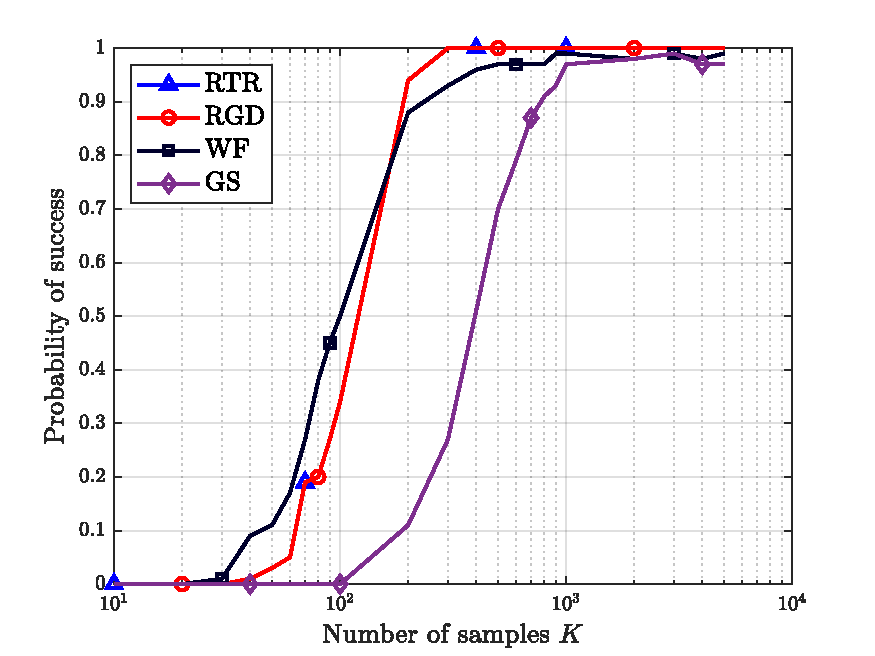
\includegraphics[width=0.8\linewidth]{./figs/rocma_figs/ROCMA_MSR_TI_QgSt_success_4QAM_L=4_M=8_J=4_nSim_100.pdf}
		% 		\caption{QPSK, $M\times L = 8\times4$.}\label{rocma:fig:CMA_ROCMA_success_8x4_4qam}	
		% 	\end{subfigure}
	% 	\begin{subfigure}{\linewidth}
		% 	\centering
		% 	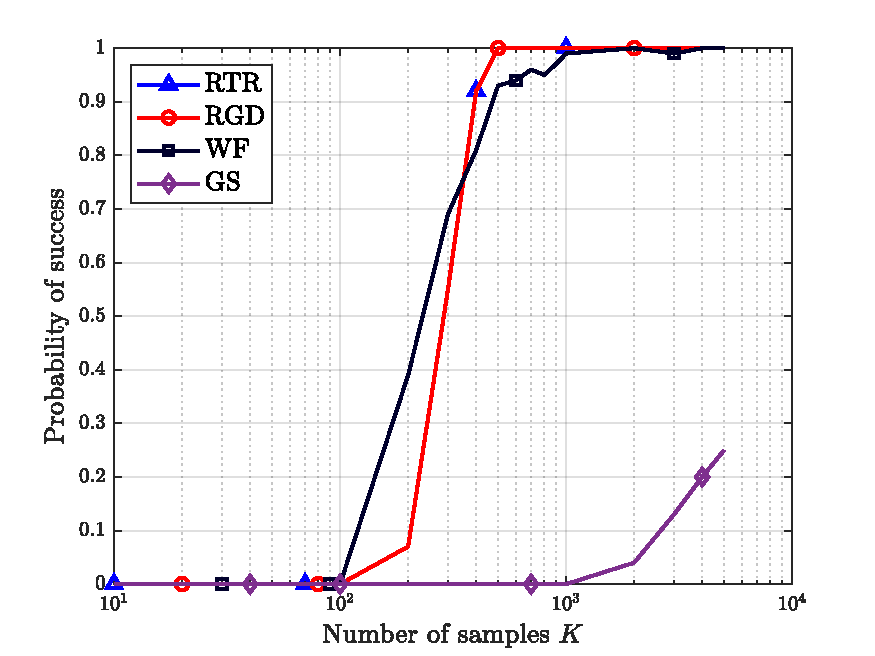
\includegraphics[width=0.8\linewidth]{./figs/rocma_figs/ROCMA_MSR_TI_QgSt_success_4QAM_L=8_M=16_J=8_nSim_100.pdf}
		% 		\caption{QPSK, $M\times L = 16\times8$.}\label{rocma:fig:CMA_ROCMA_success_16x8_4qam}		
		% 	\end{subfigure}\\
	% 	\begin{subfigure}{\linewidth}
		% 	\centering
		%     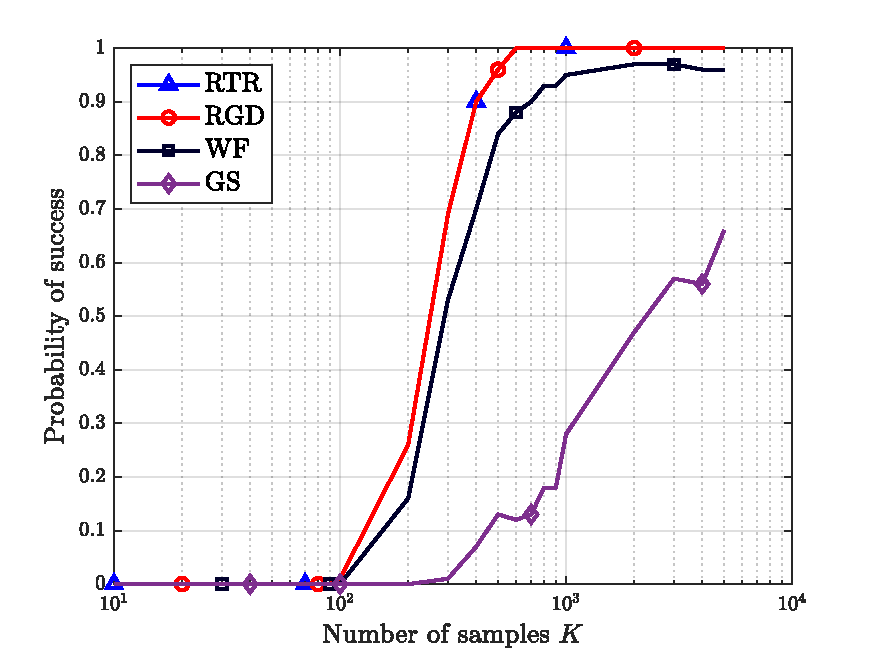
\includegraphics[width=0.8\linewidth]{./figs/rocma_figs/ROCMA_MSR_TI_QgSt_success_16QAM_L=4_M=8_J=4_nSim_100.pdf}
		% 		\caption{16-QAM, $M\times L = 8\times4$.}\label{rocma:fig:CMA_ROCMA_success_8x4_16qam}
		% 	\end{subfigure}
	% 	\begin{subfigure}{\linewidth}
		% 	\centering
		% 	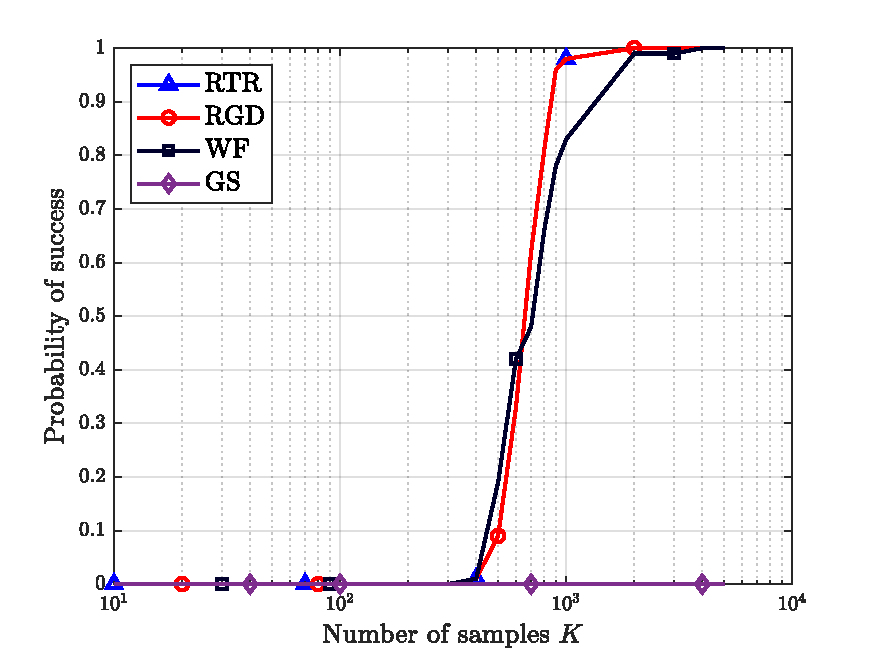
\includegraphics[width=0.8\linewidth]{./figs/rocma_figs/ROCMA_MSR_TI_QgSt_success_16QAM_L=8_M=16_J=8_nSim_100.pdf}
		% 		\caption{16-QAM, $M\times L = 16\times8$.}\label{rocma:fig:CMA_ROCMA_success_16x8_16qam}
		% 	\end{subfigure}
	% 	\caption{Probability of successful recovery of all detected demixers vs. number of samples $K$.}
	% 	\label{rocma:fig:CMA_ROCMA_success}
	% \end{figure}
%code for a 2x2 layout
\begin{figure}[htp]
	\centering
	\begin{subfigure}{0.48\linewidth}
		\centering
		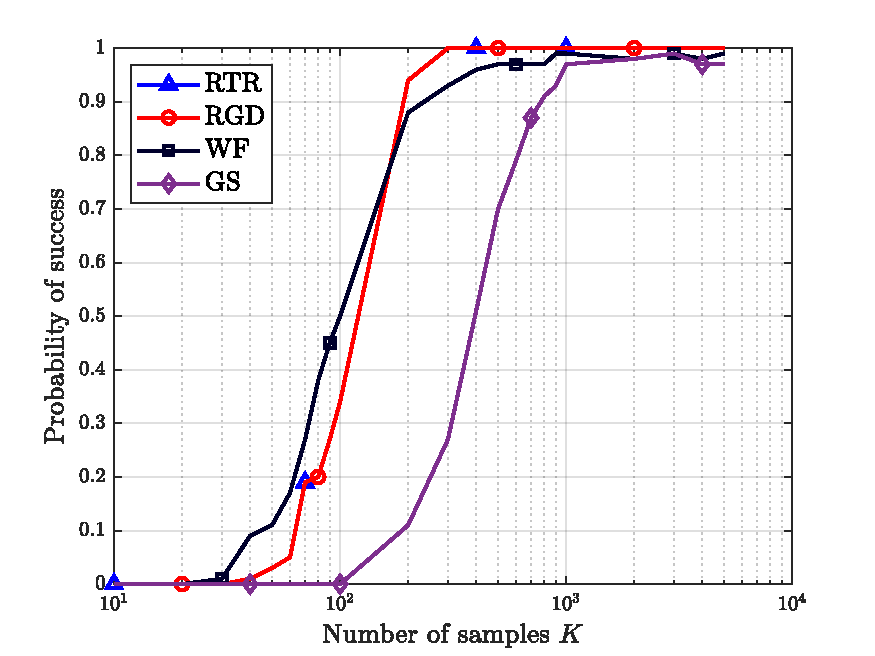
\includegraphics[width=0.95\linewidth]{./figs/rocma_figs/ROCMA_MSR_TI_QgSt_success_4QAM_L=4_M=8_J=4_nSim_100.pdf}
		\caption{QPSK, $M\times L = 8\times4$.}\label{rocma:fig:CMA_ROCMA_success_8x4_4qam}	
	\end{subfigure}
	\begin{subfigure}{0.48\linewidth}
		\centering
		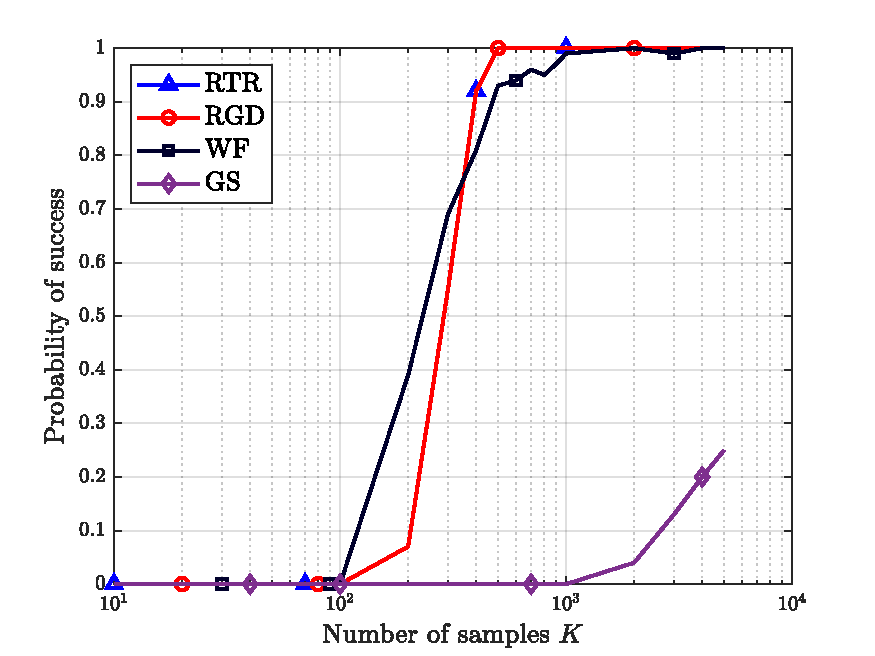
\includegraphics[width=0.95\linewidth]{./figs/rocma_figs/ROCMA_MSR_TI_QgSt_success_4QAM_L=8_M=16_J=8_nSim_100.pdf}
		\caption{QPSK, $M\times L = 16\times8$.}\label{rocma:fig:CMA_ROCMA_success_16x8_4qam}		
	\end{subfigure}\\
	\begin{subfigure}{0.48\linewidth}
		\centering
		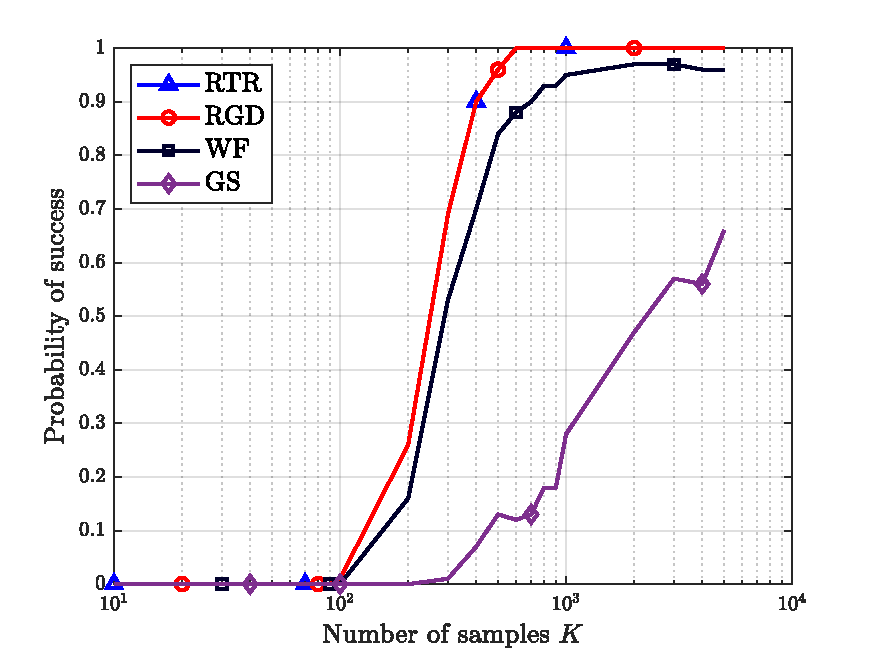
\includegraphics[width=0.95\linewidth]{./figs/rocma_figs/ROCMA_MSR_TI_QgSt_success_16QAM_L=4_M=8_J=4_nSim_100.pdf}
		\caption{16-QAM, $M\times L = 8\times4$.}\label{rocma:fig:CMA_ROCMA_success_8x4_16qam}
	\end{subfigure}
	\begin{subfigure}{0.48\linewidth}
		\centering							
		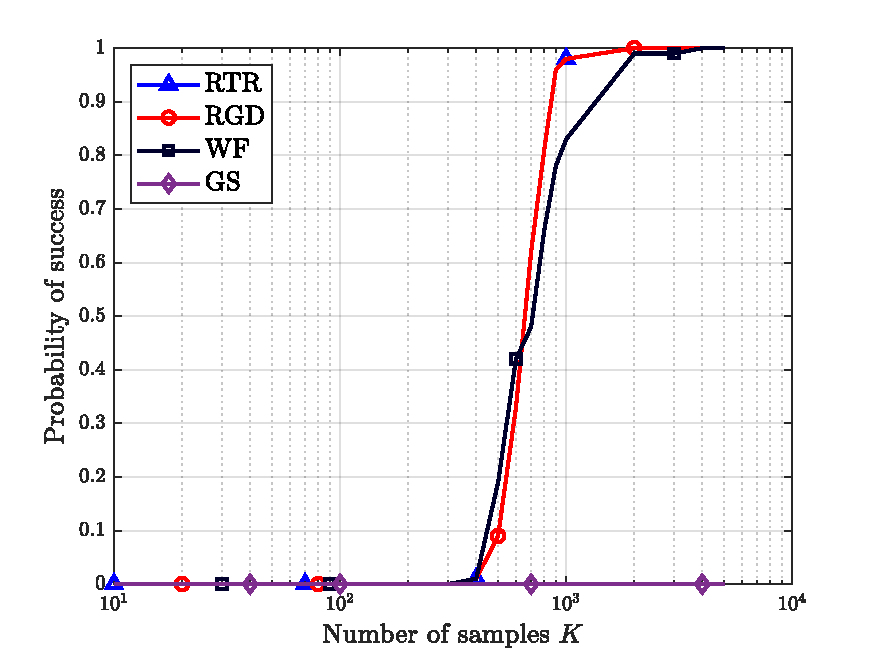
\includegraphics[width=0.95\linewidth]{./figs/rocma_figs/ROCMA_MSR_TI_QgSt_success_16QAM_L=8_M=16_J=8_nSim_100.pdf}
		\caption{16-QAM, $M\times L = 16\times8$.}\label{rocma:fig:CMA_ROCMA_success_16x8_16qam}
	\end{subfigure}
	\caption{Probability of successful recovery of all detected demixers vs. number of samples.}
	\label{rocma:fig:CMA_ROCMA_success}
\end{figure}

Testing a larger system using QPSK, 
results from Figure~\ref{rocma:fig:CMA_ROCMA_success_16x8_4qam}
demonstrate similar relative performance
by RTR, RGD and WF, 
requiring $500$ and $1000$ samples to achieve over 99\% probability of success. 
The GS-CMA demixer, however, is much more
sensitive to problem size, and struggles to jointly recover all signals even with 5000
received data samples.

We now consider the more challenging
case of 16-QAM source signals. 
Figures~\ref{rocma:fig:CMA_ROCMA_success_8x4_16qam} and~\ref{rocma:fig:CMA_ROCMA_success_16x8_16qam} respectively provide the results for
problem size of $8\times 4$ and $16\times 8$.
The test results 
show that the
two Riemann methods (RTR and RGD) again
achieve high probability of
successful signal recovery, now requiring 
only $600$ and $2000$ samples, respectively
for near 100\% success rate. The WF algorithm 
is less successful in comparison,
requiring at least $2000$ samples to achieve more than $95\%$ of success probability. 
On other other hand, 
GS-CMA only achieves $60\%$ probability of success for 16-QAM 
for the smaller $8\times 4$ system size. 
For the more complex system of size
$16\times 8$, GS-CMA
in fact is unable to recover all 8 detected sources under the stated simulation settings. 
Indeed, this phenomenon was anticipated by \cite{Nguyen1997}. 
Since GS-CMA relies on sequential Gram-Schmidt orthogonalization for signal separation, 
error propagation can lead to weaker interference suppression. As the $\ell$-th demixer relies on all previous demixers in order to isolate a different signal, 
GS-CMA becomes increasingly more vulnerable to error propagation with increasing number of signals.

Overall, both proposed Riemann algorithms
(RTR and RGD) demonstrate strong performance across different modulations and system sizes under test than their Euclidean counterparts.
WF-CMA still shows high probability of  successful recovery, albeit at the
cost of more samples than RTR or RGD. 
GS-CMA, on the other hand, struggles
against moderately large system sizes or
higher-order modulations.


\subsection{Computation and Interference Rejection}\label{rocma:sim:complexity}
For the purposes of signal recovery, computation complexity must be jointly
analyzed with respect to the achieved
level of interference rejection in
recovered signals. 
For this reason, in the following presentation
we show how well our proposed methods (RTR and RGD) work in terms of both interference rejection and computational load.
We also provide benchmark
comparison with the two algorithms (WF and GS).

We first investigate
algorithm runtime (``wall-clock'' time). Runtime depends on computer, platform and code implementation. Thus, runtime comparison 
alone may not fully capture true
algorithm runtime. 
To mitigate this possible bias, 
we let
all source codes for RTR, RGD and WF utilize the same Manopt structure and libraries. GS-CMA, on the other hand, uses a direct implementation using the fastest routines available (matrix products, etc.)
for each iteration.

Figure~\ref{rocma:fig:CMA_ROCMA_runtime} depicts the average interference rejection over all runs of the algorithms with respect to their runtime, for a fixed number of samples $K=2000$. From the results of
all tested modulation schemes and system sizes, both RGD and RTR, by exploiting
the proposed geometry, 
are faster than GS by at least 4 times, and
are faster than WF by an order of magnitude.
Such advantage is consistent 
across nearly all tested modulation schemes and system sizes. 
Moreover, RTR and RGD exhibit similar runtime across modulations, and require about double the time to converge in the larger system
of $16\times 8$, which contains 2 times more sources and antennas (Figures~\ref{rocma:fig:CMA_ROCMA_runtime_16x8_4qam} and~\ref{rocma:fig:CMA_ROCMA_runtime_16x8_16qam}). 
There are some modest differences
between the two Riemann solvers. In 
particular, RGD converges slightly faster initially to achieve moderate interference mitigation of
approximately -15dB. For higher
interference rejection, both RGD and RTR 
show similar runtime complexity. 
\begin{figure}[ht]
	\centering
	\begin{subfigure}{0.48\linewidth}
		\centering
		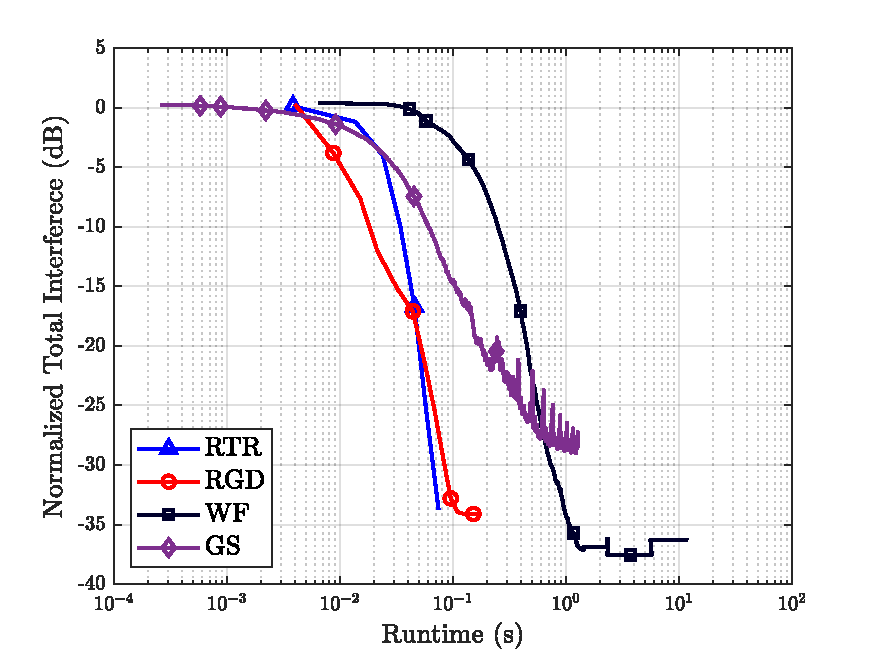
\includegraphics[width=0.95\linewidth]{./figs/rocma_figs/ROCMA_MSR_TI_QgSt_runtime_4QAM_L=4_M=8_J=4_nSim_100.pdf}
		\caption{QPSK, $M\times L = 8\times4$.}\label{rocma:fig:CMA_ROCMA_runtime_8x4_4qam}
	\end{subfigure}
	\begin{subfigure}{0.48\linewidth}
		\centering
		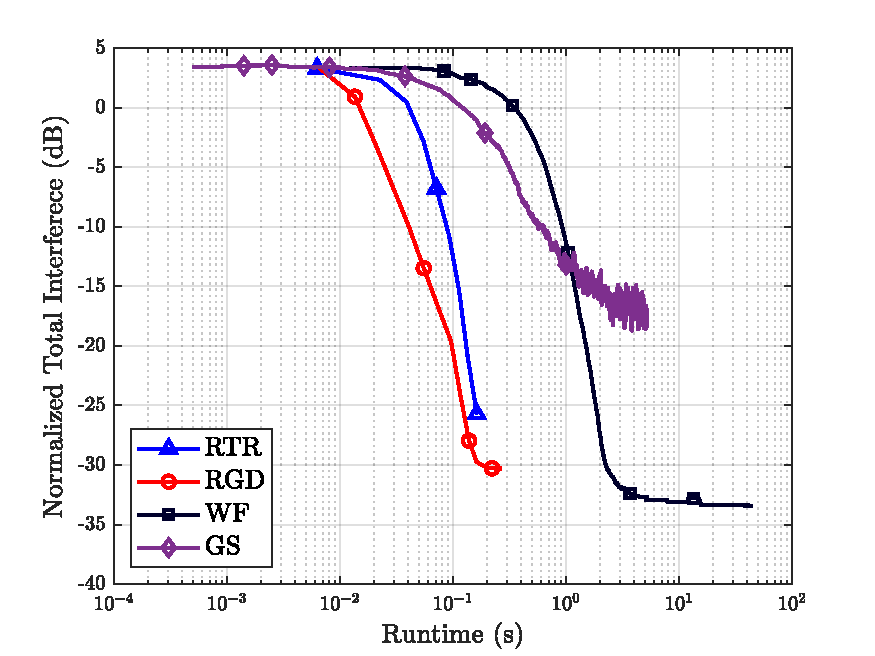
\includegraphics[width=0.95\linewidth]{./figs/rocma_figs/ROCMA_MSR_TI_QgSt_runtime_4QAM_L=8_M=16_J=8_nSim_100.pdf}
		\caption{QPSK, $M\times L = 16\times8$.}\label{rocma:fig:CMA_ROCMA_runtime_16x8_4qam}		
	\end{subfigure}
	\begin{subfigure}{0.48\linewidth}
		\centering
		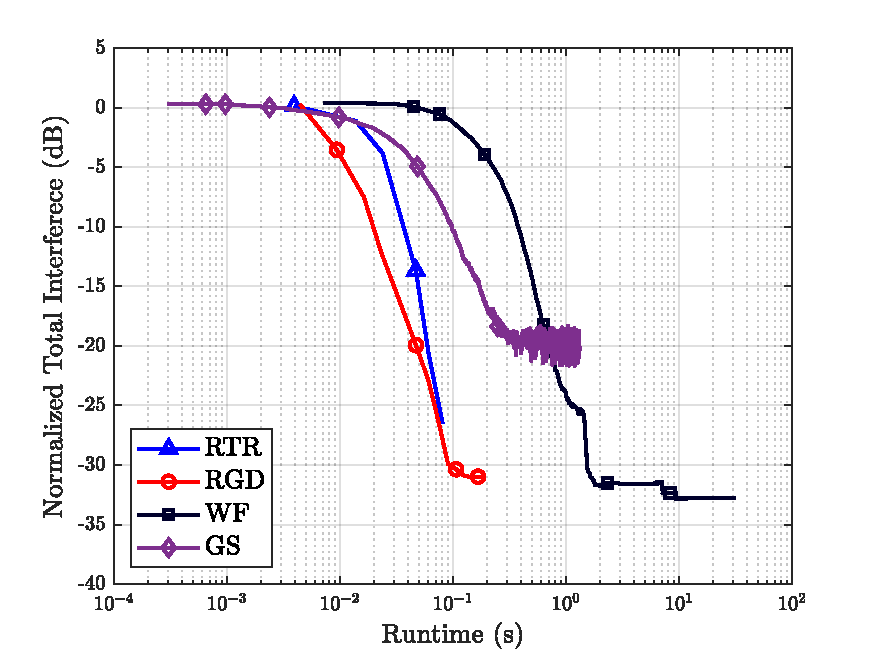
\includegraphics[width=0.95\linewidth]{./figs/rocma_figs/ROCMA_MSR_TI_QgSt_runtime_16QAM_L=4_M=8_J=4_nSim_100.pdf}
		\caption{16-QAM, $M\times L = 8\times4$.}\label{rocma:fig:CMA_ROCMA_runtime_8x4_16qam}
	\end{subfigure}
	\begin{subfigure}{0.48\linewidth}
		\centering
		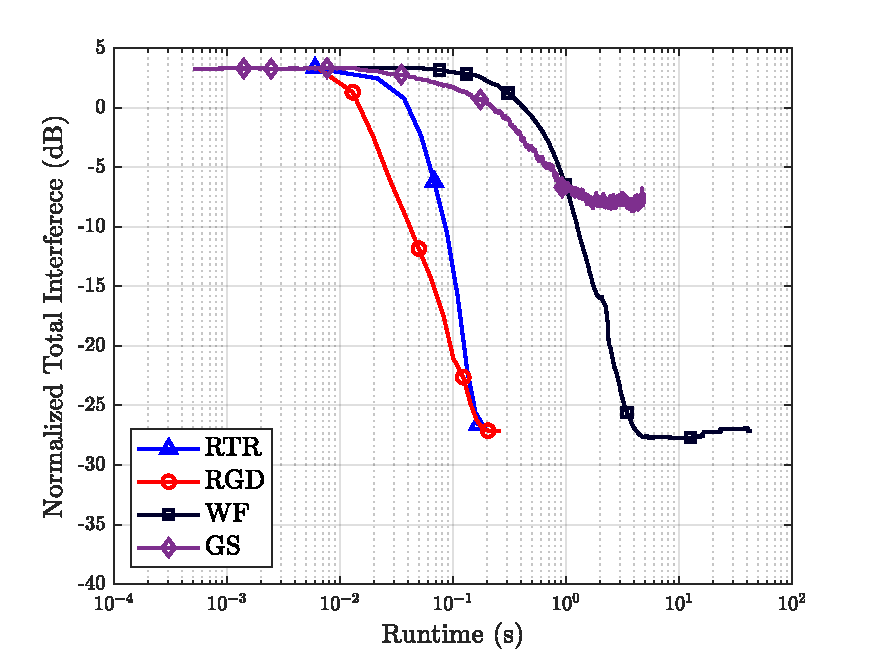
\includegraphics[width=0.95\linewidth]{./figs/rocma_figs/ROCMA_MSR_TI_QgSt_runtime_16QAM_L=8_M=16_J=8_nSim_100.pdf}
		\caption{16-QAM, $M\times L = 16\times8$.}\label{rocma:fig:CMA_ROCMA_runtime_16x8_16qam}		
	\end{subfigure}
	\caption{Average total interference for all detected demixers vs. runtime.}
	\label{rocma:fig:CMA_ROCMA_runtime}
\end{figure}

WF-CMA exhibits a similar efficacy in terms
of interference rejection, but it does
require longer runtime to achieve a particular level of interference rejection.  On the other hand, GS-CMA requires more runtime to
converge than the Riemannian methods across all tested scenarios. Moreover, GS-CMA is less effective in interference mitigation, particularly
for more complex source signals of 16-QAM, as shown in Figure~\ref{rocma:fig:CMA_ROCMA_runtime_8x4_16qam} 
and Figure~\ref{rocma:fig:CMA_ROCMA_runtime_16x8_16qam}.
From the test results, it is evident that
GS-CMA stalls in terms of interference rejection
and additional iterations do not improve 
the performance of 
interference rejection. This phenomenon is
consistent with the discussion of error propagation in sequential orthogonalization of the GS-CMA
approach. The performance loss of GS-CMA
becomes more severe with increasing modulation 
and system size, e.g. is about -30dB of interference for QPSK signals and a $8\times4$ system (Figure~\ref{rocma:fig:CMA_ROCMA_runtime_8x4_4qam}), but is less than -10dB for 16QAM and $16\times8$ system (Figure~\ref{rocma:fig:CMA_ROCMA_runtime_16x8_16qam}). 


To address the potential bias of over-reliance on runtime when analyzing computation complexity, we also compare the algorithm behavior respect to \emph{oracle calls}, that is, the total 
number of cost function, gradient, Hessian and GS orthogonalization calls/evaluations of each algorithm. 
These operations are dominant contributors to total computational complexity, they act as a proxy for platform-independent computational load assessment.
Recall that GS-CMA uses only one sample per gradient update and its orthogonalization does not increase with the number of samples, we normalize the number of oracles calls by $K$ in order to provide a fair comparison with the other methods, that use sample averages in all its oracle calls.

Figure~\ref{rocma:fig:CMA_ROCMA_oracles} shows the average achieved NTI of each algorithm with respect to their oracle calls, for a fixed number of samples $K=2000$. 
As seen in previous comparisons, RTR and RGD have similar computational cost. 
Across the tested modulations and system sizes, both RGD and RTR require at least an order of magnitude fewer function computations than WF-CMA to achieve 20dB of interference mitigation. 
Even if we account for their larger computational complexity per iteration than WF or GS, the total cost of every algorithm is dominated by the number of iterations, and RTR and RGD incur significantly lower total computational load than WF-CMA. 
WF-CMA shows good interference rejection power, but requires about 10-20 times more oracle computations than the Riemannian methods to achieve equal levels of interference mitigation.
\begin{figure}[ht]
	\centering
	\begin{subfigure}{0.48\linewidth}
		\centering
		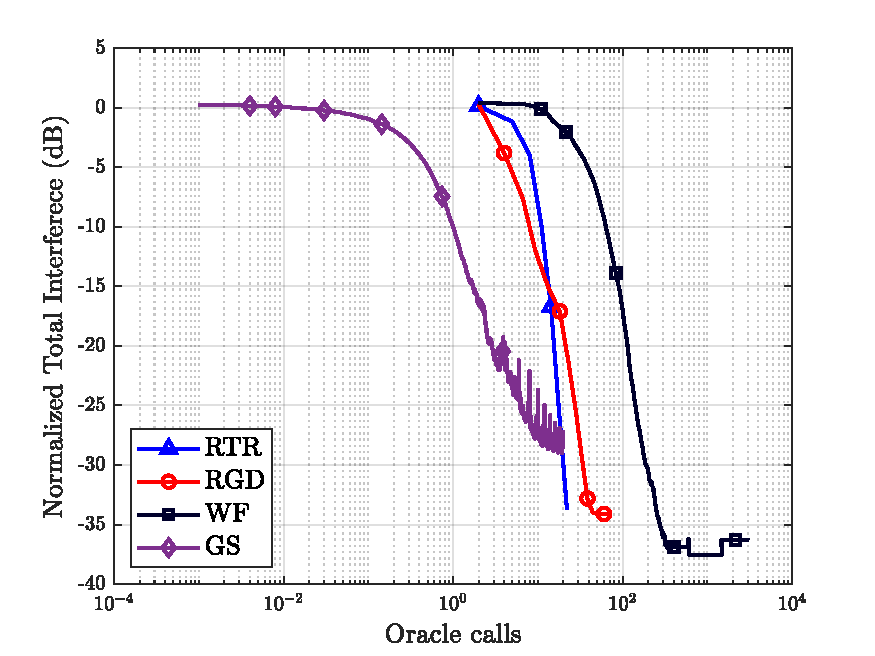
\includegraphics[width=0.95\linewidth]{./figs/rocma_figs/ROCMA_MSR_TI_QgSt_oracles_4QAM_L=4_M=8_J=4_nSim_100.pdf}
		\caption{QPSK, $M\times L = 8\times4$.}\label{rocma:fig:CMA_ROCMA_oracles_8x4_4qam}
	\end{subfigure}
	\begin{subfigure}{0.48\linewidth}
		\centering
		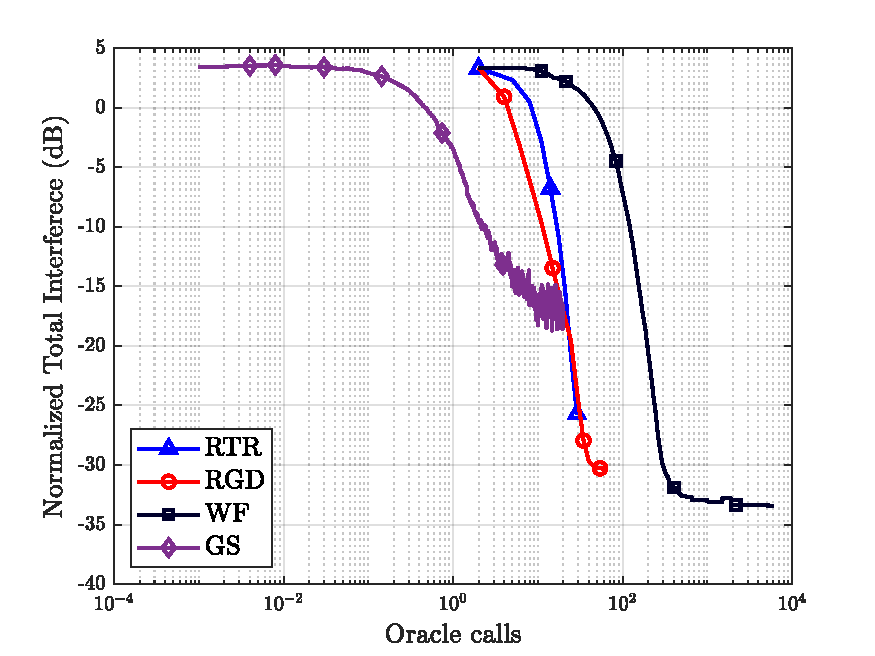
\includegraphics[width=0.95\linewidth]{./figs/rocma_figs/ROCMA_MSR_TI_QgSt_oracles_4QAM_L=8_M=16_J=8_nSim_100.pdf}
		\caption{QPSK, $M\times L = 16\times8$.}\label{rocma:fig:CMA_ROCMA_oracles_16x8_4qam}
	\end{subfigure}
	\begin{subfigure}{0.48\linewidth}
		\centering
		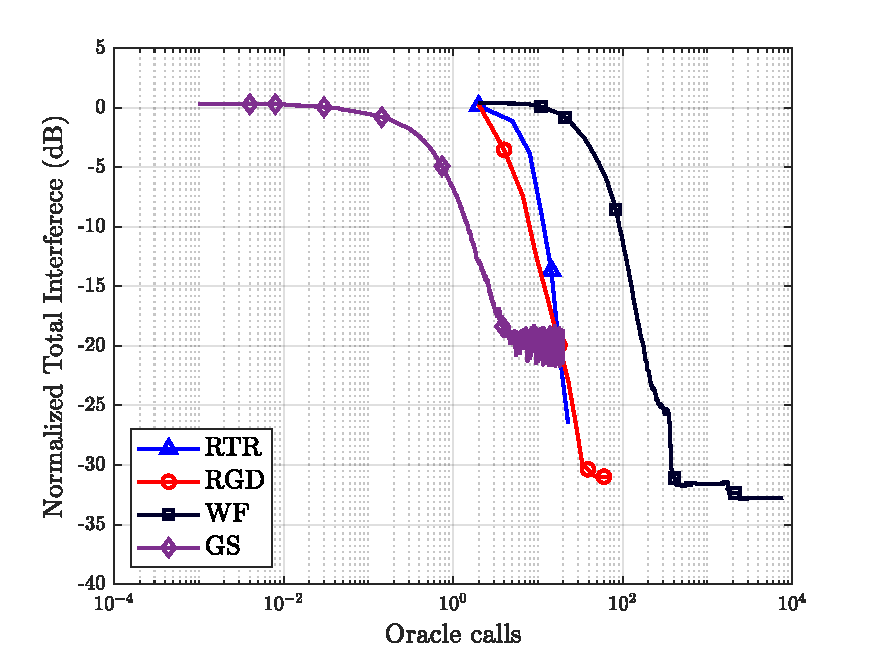
\includegraphics[width=0.95\linewidth]{./figs/rocma_figs/ROCMA_MSR_TI_QgSt_oracles_16QAM_L=4_M=8_J=4_nSim_100.pdf}
		\caption{16-QAM, $M\times L = 8\times4$.}\label{rocma:fig:CMA_ROCMA_oracles_8x4_16qam}
	\end{subfigure}
	\begin{subfigure}{0.48\linewidth}
		\centering
		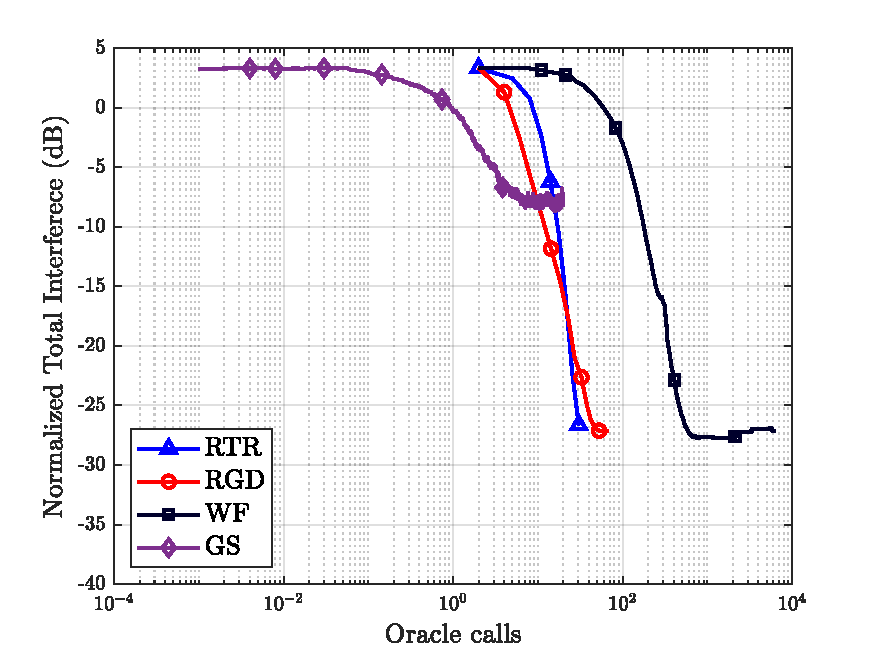
\includegraphics[width=0.95\linewidth]{./figs/rocma_figs/ROCMA_MSR_TI_QgSt_oracles_16QAM_L=8_M=16_J=8_nSim_100.pdf}
		\caption{16-QAM, $M\times L = 16\times8$.}\label{rocma:fig:CMA_ROCMA_oracles_16x8_16qam}		
	\end{subfigure}
	\caption{Average total interference for all detected demixers vs. oracle calls. }
	\label{rocma:fig:CMA_ROCMA_oracles}
\end{figure}

As expected, GS is the least complex algorithm owing to its simply stochastic gradient update using only one sample in each iteration. 
At an average interference suppression of 20dB, the computational cost of GS is about 5-8 times lower than the Riemannian methods, as seen in Figs~\ref{rocma:fig:CMA_ROCMA_oracles_8x4_4qam}-\ref{rocma:fig:CMA_ROCMA_oracles_8x4_16qam}.
However, the sequential nature of the GS-CMA leads to poorer interference rejection, particularly for higher-dimensional QAM constellation and/or larger system sizes. 
In comparison, the proposed Riemann algorithms can achieve substantially better performance of signal recovery with only a modest increase of computation complexity. 
Exploiting Riemannian geometry provides a good complexity-efficacy tradeoff. 

\section{Summary}
In this chapter, we investigated an alternative formulation for CMA-based signal recovery based on Riemannian manifolds. We avoided regularization by imposing constraints in the original optimization problem. Then, we developed a Riemannian geometry that encodes the orthogonality requirement of distinct source signals, and thus we rewrite the CMA problem as an unconstrained optimization problem over our proposed manifold geometry. We leveraged Riemannian optimization techniques to solve this problem without the need for parameter tuning or special initialization, and furthermore, provided theoretical convergence guarantees with high probability under mild conditions. Our numerical test corroborated these claims when compared with traditional CMA solutions, showing lower requirement of sample size, computations and runtime.